\chapter{Clustering \label{chapter:clustering}}

Our discussions so far have focused on the problem of supervised learning, in which we create a mapping between a set of inputs and an output. In this chapter, we turn our attention to the problem of \textbf{unsupervised learning}, in which our goal is to uncover hidden structure in a dataset. There is no ``special'' outcome variable in these types of problems. Way back in Chapter~\ref{chapter:overview}, examples 7, 8, and 14 were examples of unsupervised learning problems.

%%%%%%%%%%%%%%%%%%%%%%%%%%%%%%%%%%%%%%%%%%%%%%%%%%%%%%%%%%%%%%%%%%%%%%%%%%%%%%%%

\section{A Thought Experiment: Flow Cytometry Data}

Imagine you have data on 500 cells from two different cell lines. For each cell, you record the fluorescence intensity of two different biomarkers, biomarker 1 ($x_1$) and biomarker 2 ($x_2$). The data are shown below. 

\begin{center}
    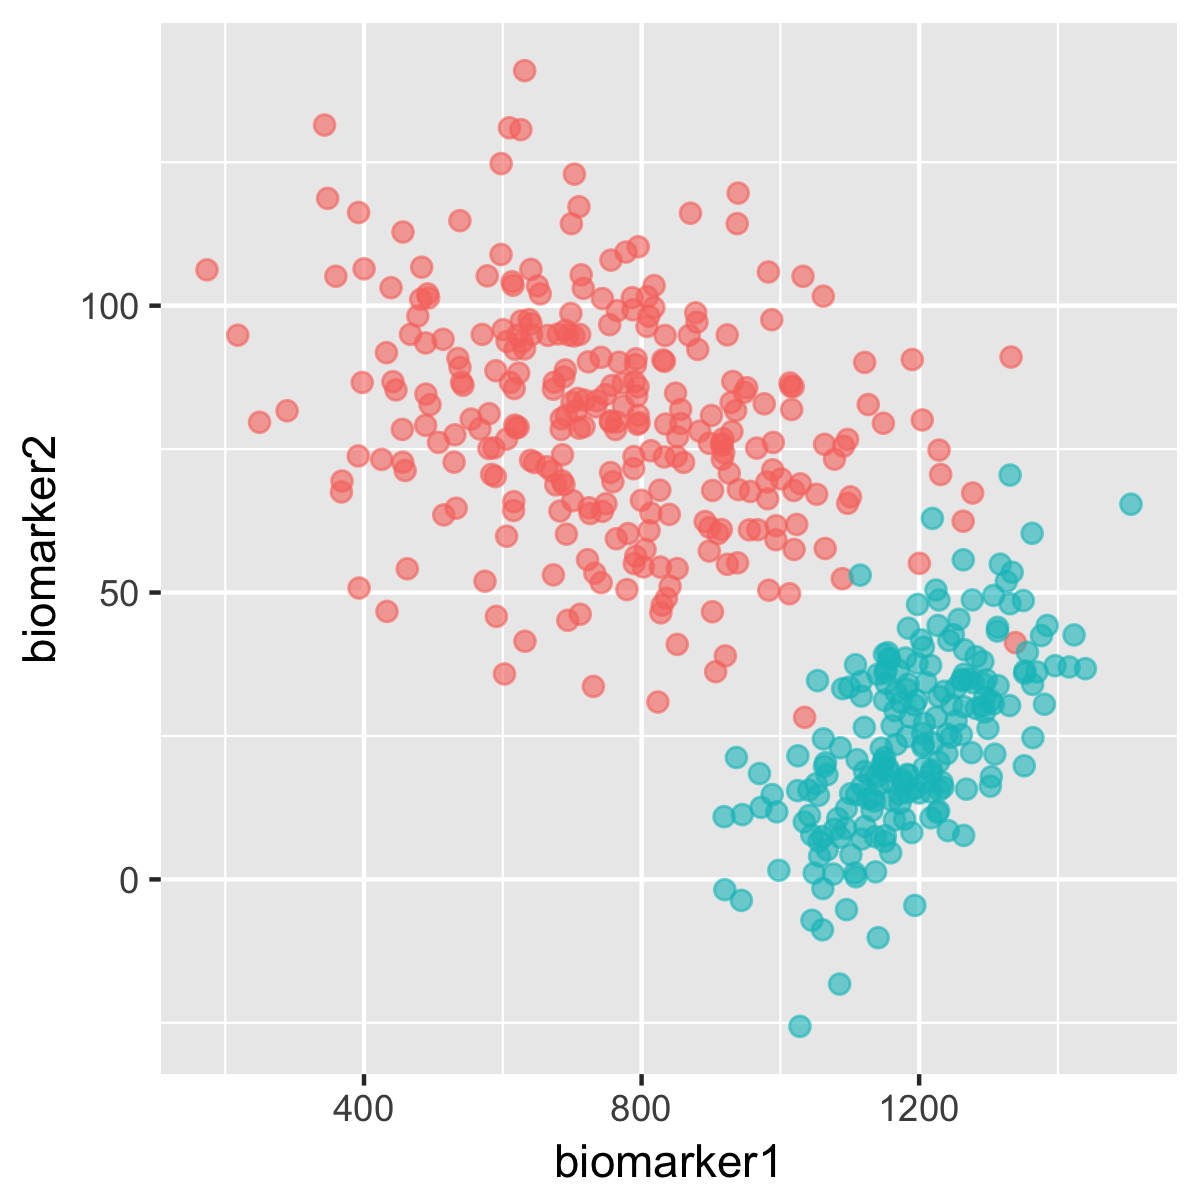
\includegraphics[width=0.7\textwidth]{img/biomarker-data-big-labels.png}
    \par\bigskip
    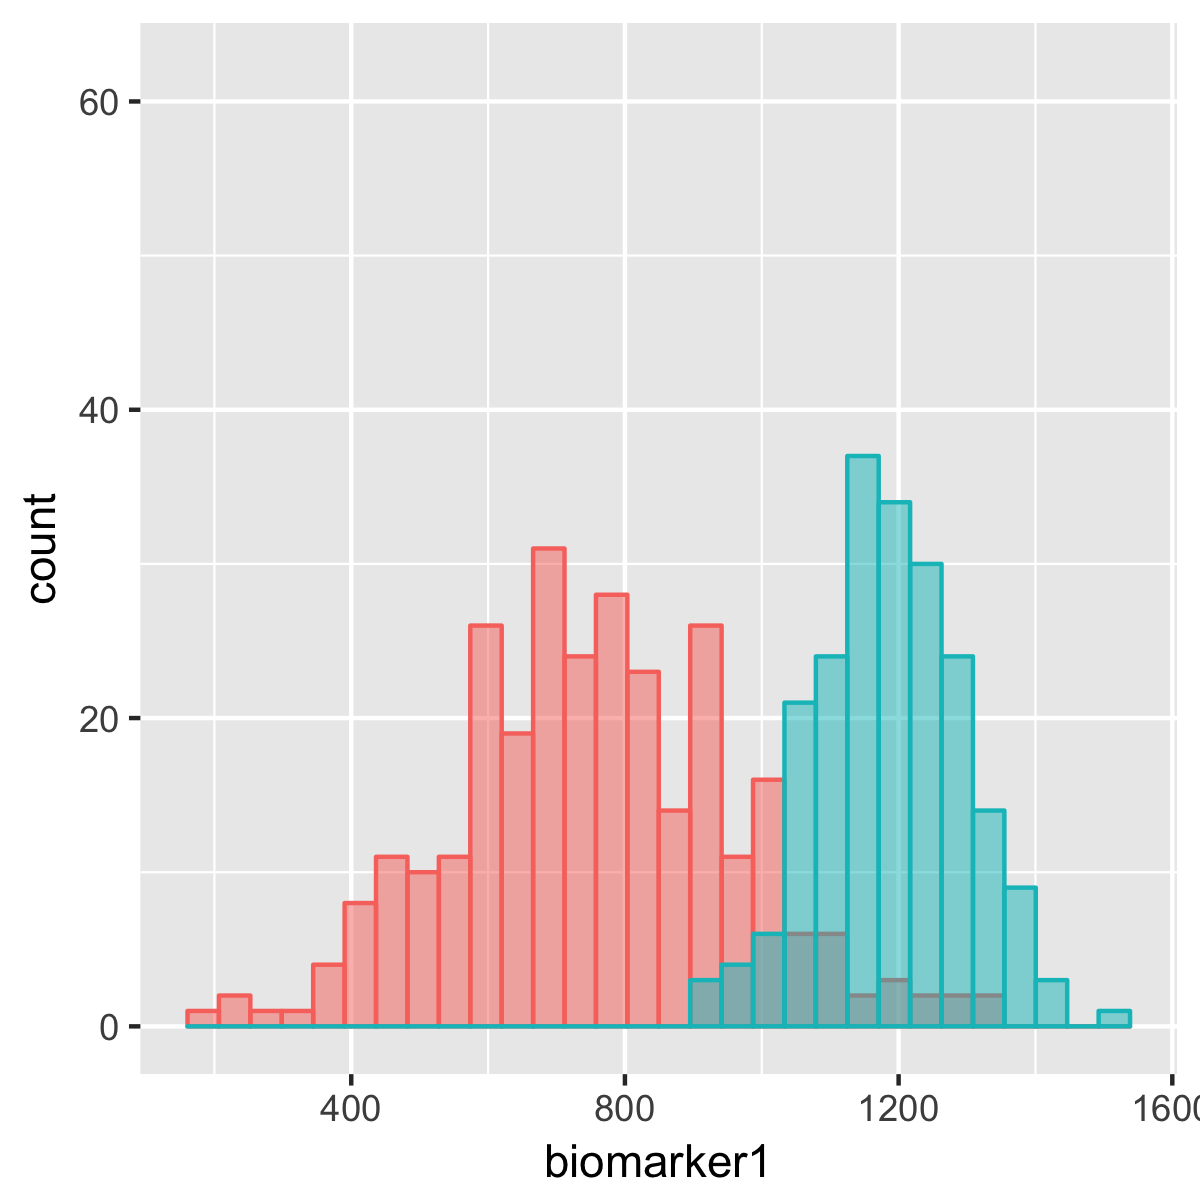
\includegraphics[width=0.42\textwidth]{img/biomarker-data-biomarker1-big-labels.png} \qquad
    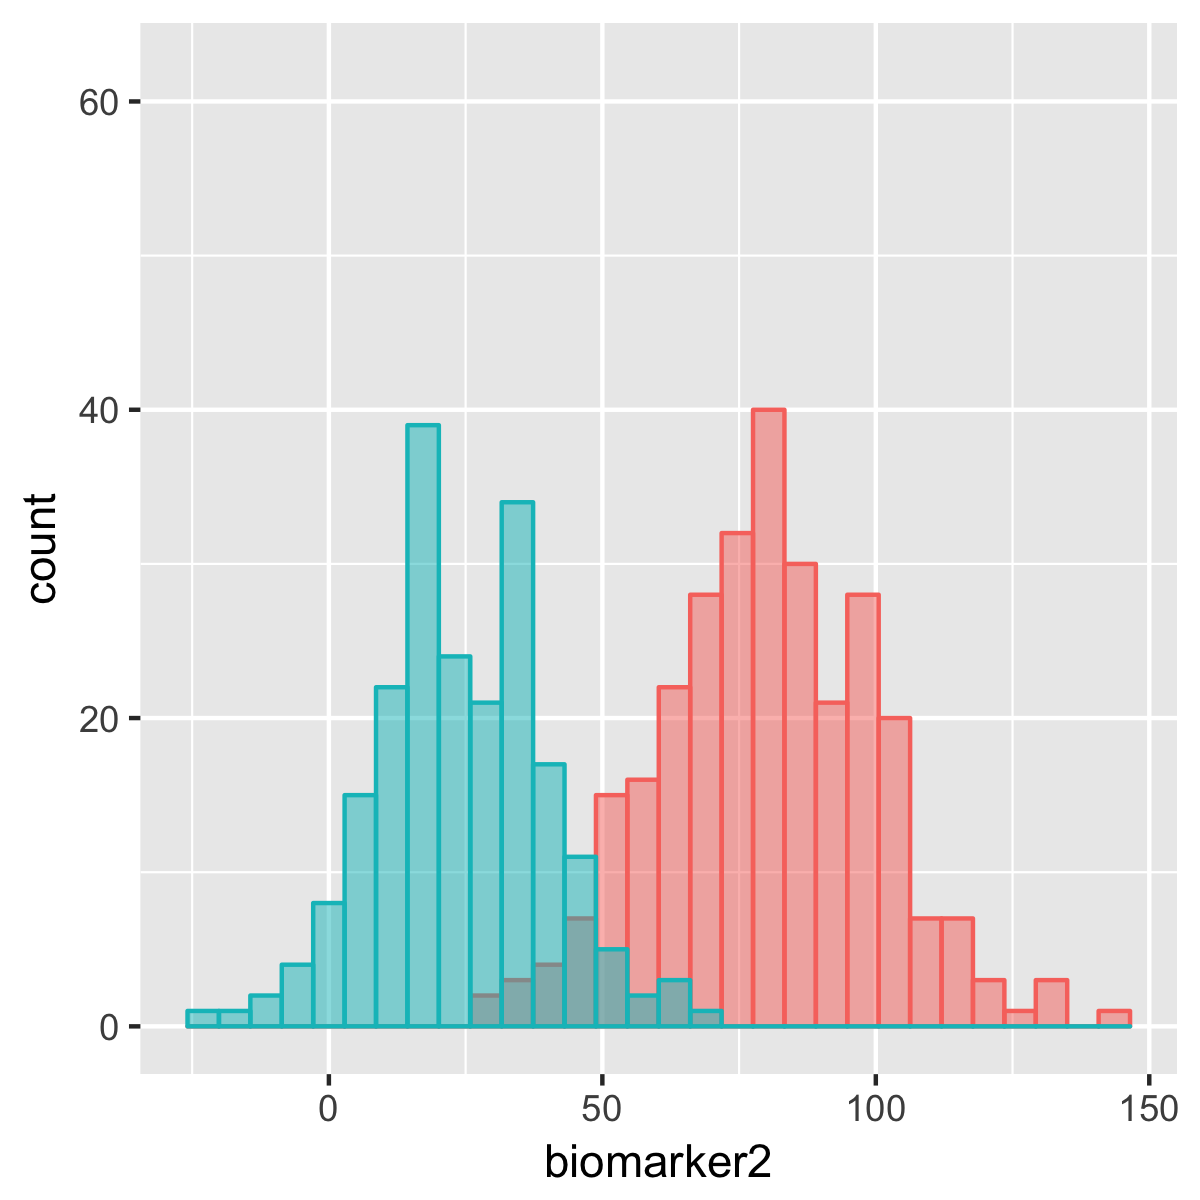
\includegraphics[width=0.42\textwidth]{img/biomarker-data-biomarker2-big-labels.png}
\end{center}

In real life, you would not have the labels for the two cell lines. You would have no idea which distribution(s) the data were drawn from or what the probabilities associated with the various distributions were. Real flow cytometry data would instead look like this:

\begin{center}
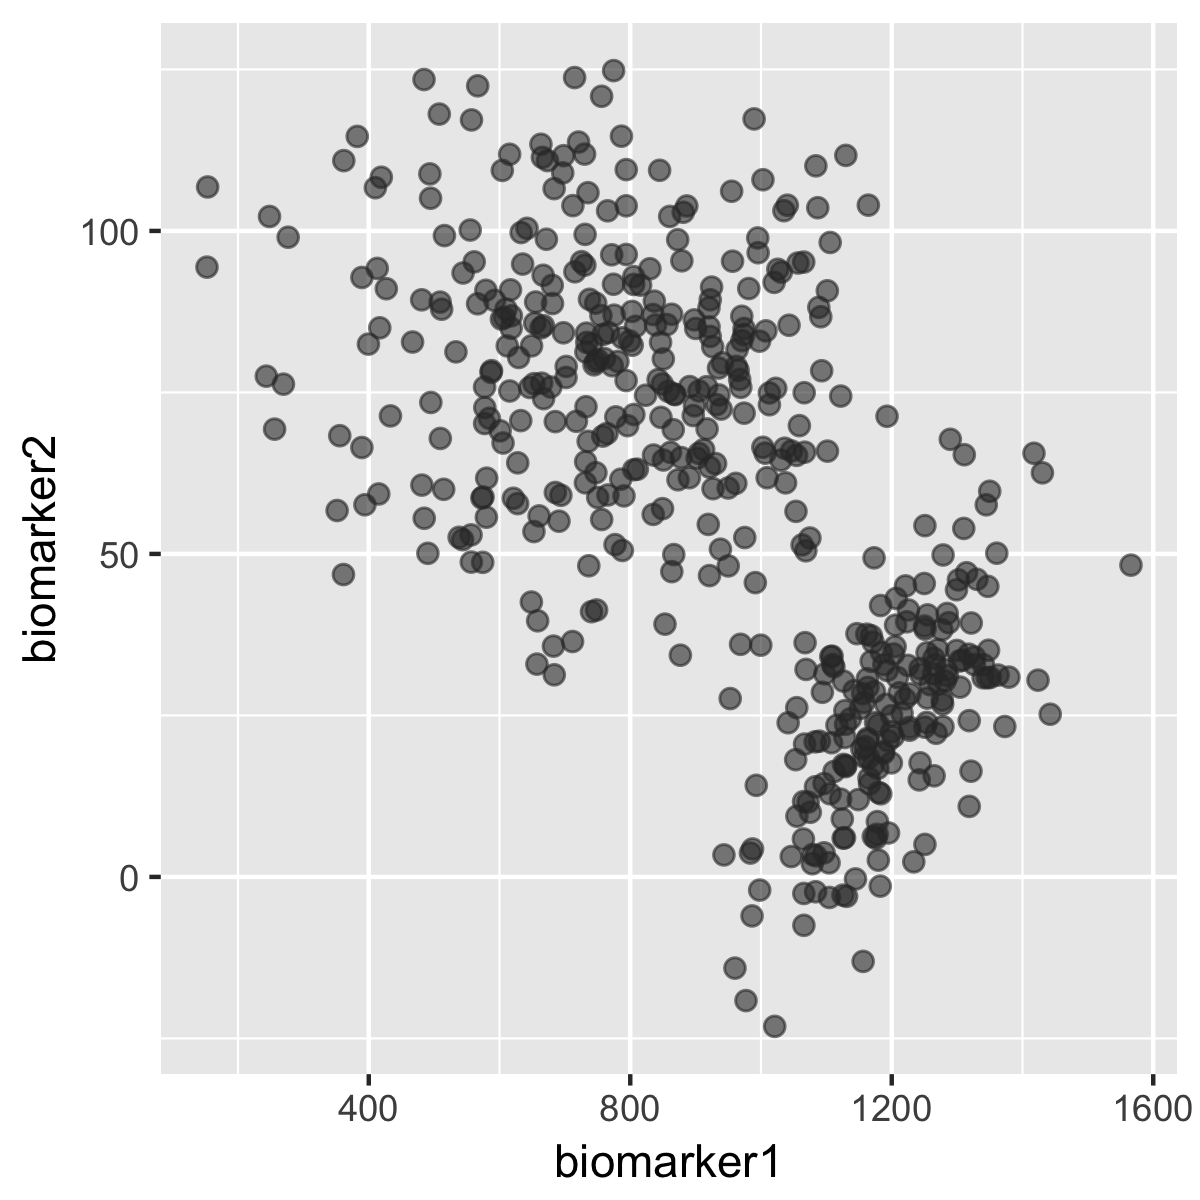
\includegraphics[width=0.7\textwidth]{img/biomarker-data-big-no-labels.png}
\end{center}

The human eye can distinguish structure in a plot like this, but it's harder to train a computer to see it, and it's even harder to prove that the structure the computer finds is real. Over the years, people have tried many different strategies.

\vspace{3mm}

\begin{question}{}
Speculate on some possible approaches for separating data that look like this into groups, or clusters. 
\end{question}

\subsection{Downsampled Dataset}

For the rest of this workshop, we need to be able to calculate things by hand, so we will downsample the flow cytometry data, above, to just $10$ datapoints. The downsampled, labeled data are shown here:

\begin{center}
\begin{tabular}{rrrc}
  \toprule
$i$ & Biomarker 1 Intensity $(x_1^{(i)})$ & Biomarker 2 Intensity $(x_2^{(i)})$ & Cell Line $(z)$ \\
  \midrule
1 & 634.83 & 110.55 & B \\ 
  2 & 650.06 & 74.22 & B \\ 
  3 & 788.24 & 81.52 & B \\ 
  4 & 771.47 & 84.98 & B \\ 
  5 & 515.81 & 91.08 & B \\ 
  6 & 1101.23 & 31.05 & A \\ 
  7 & 649.32 & 77.05 & B \\ 
  8 & 652.89 & 97.16 & B \\ 
  9 & 1183.02 & 11.73 & A \\ 
  10 & 1238.45 & 33.46 & A \\ 
   \bottomrule
\end{tabular}
\end{center}

\vspace{5mm}

\noindent Without their labels, the data look like this:

\begin{center}
\begin{tabular}{rrrc}
  \toprule
$i$ & Biomarker 1 Intensity $(x_1^{(i)})$ & Biomarker 2 Intensity $(x_2^{(i)})$ & Cell Line $(z)$ \\
  \midrule
1 & 634.83 & 110.55 \\ 
  2 & 650.06 & 74.22 \\ 
  3 & 788.24 & 81.52 \\ 
  4 & 771.47 & 84.98 \\ 
  5 & 515.81 & 91.08 \\ 
  6 & 1101.23 & 31.05 \\ 
  7 & 649.32 & 77.05 \\ 
  8 & 652.89 & 97.16 \\ 
  9 & 1183.02 & 11.73 \\ 
  10 & 1238.45 & 33.46 \\ 
   \bottomrule
\end{tabular}
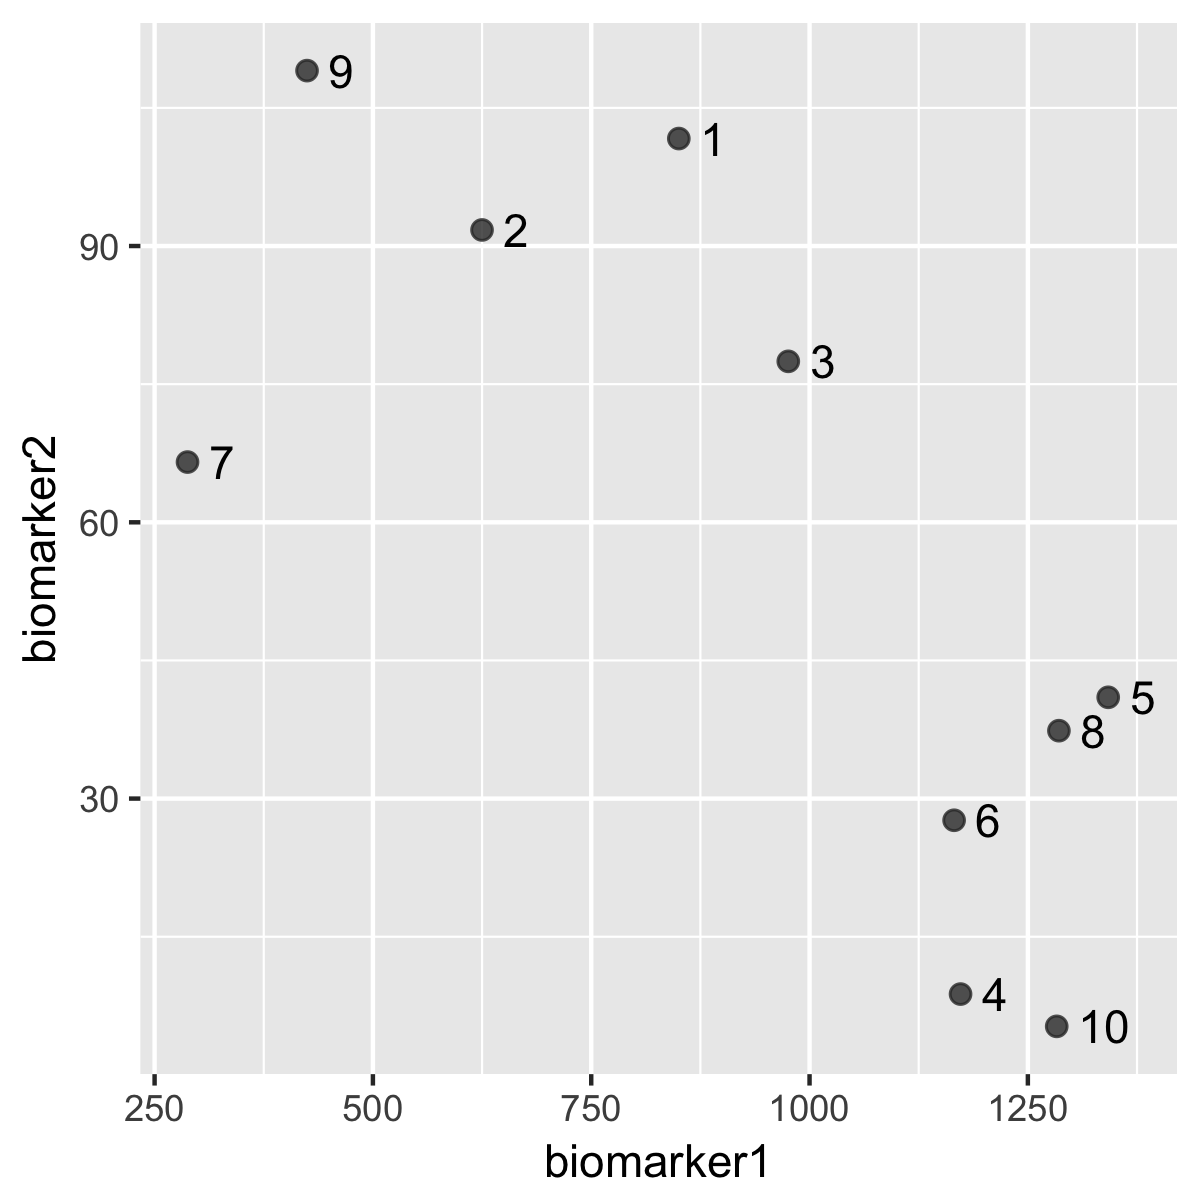
\includegraphics[width=0.7\textwidth]{img/biomarker-data-labels.png}
\end{center}

%%%%%%%%%%%%%%%%%%%%%%%%%%%%%%%%%%%%%%%%%%%%%%%%%%%%%%%%%%%%%%%%%%%

\section{K-Means}

Let's first consider a very simple unsupervised machine learning algorithm called \textbf{K-means}. The goal of K-means is to cluster [unlabeled] data into groups so that the distances between points within a group are minimized.

Assume you have a dataset $\{ x^{(1)}, x^{(2)}, \dots, x^{(n)} \}$, where each vector $x^{(i)}$ is of length $p$, and you want to cluster these $n$ vectors into $K$ distinct groups. Here is the K-means algorithm:
\begin{enumerate}
\item Assign each of the $n$ datapoints to a random cluster. You can do this one of three ways: 
	\begin{enumerate}
	\item[(1)] Choose a random cluster for each point independently. 
	\item[(2)] Choose $K$ initial points to be the cluster centers.
	\item[(3)] Choose $K$ initial points uniformly within the feature space (not necessarily data point locations) to be the cluster centers. 
	\end{enumerate}
	After the initial cluster assignments are made, proceed to the update step, below.
\item \textbf{Assignment step.} Assign each point to the cluster whose mean is the closest, using Euclidean distance. Mathematically:
$$ c_i^{(t)} := \text{argmin}_j \| x^{(i)} - \mu_j \| $$
where we note that the distance is given by the $L_2$, or Euclidean, norm.
\item \textbf{Update step.} Calculate the means to be the centroids of the points in the clusters.
$$ \mu_j^{(t)} := \frac{\sum_{i=1}^n x^{(i)} \cdot \mathbb{I} \left\{ c^{(i)} = j \right\}}{\sum_{i=1}^n \mathbb{I} \left\{ c^{(i)} = j \right\}} $$
\item Repeat Steps 2 and 3 until no points change clusters (or until convergence). 
\end{enumerate}

\vspace{3mm}

\begin{question}{}
Which supervised learning algorithm does this remind you of? What is different between K-means and this algorithm?
\end{question}

\begin{question}{}
Below is our unlabeled, downsampled flow cytometry dataset. Cluster it into two groups using K-means. You can initialize your clusters however you want. (Note: Assume that the data were standardized in advance so that the spacing between the white lines equals one ``unit'' for both biomarker 1 and biomarker 2.)
\begin{center}
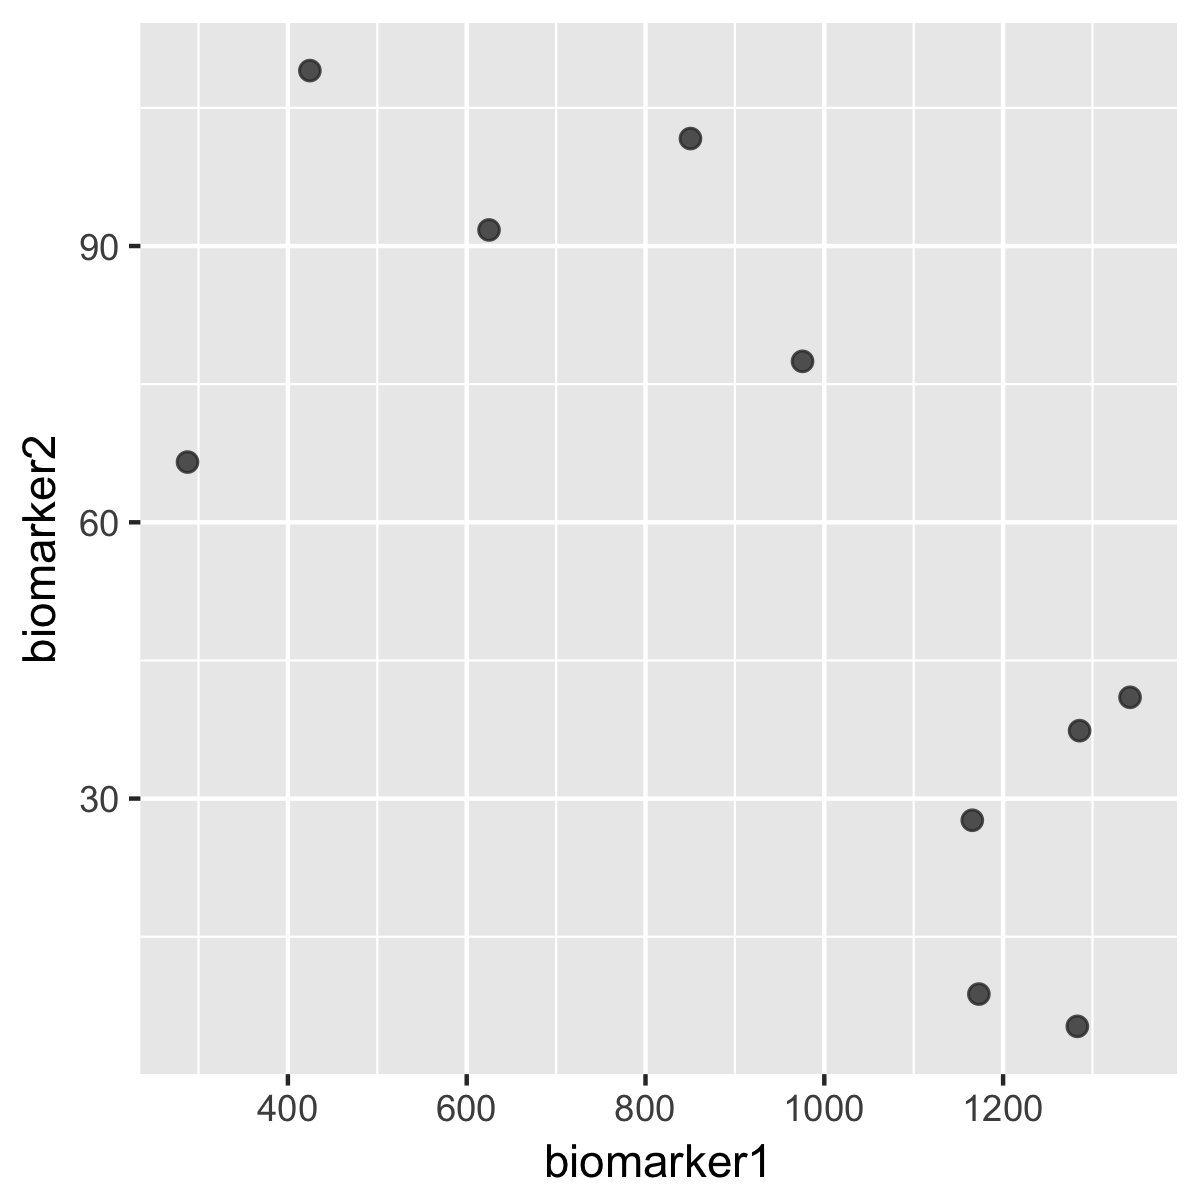
\includegraphics[width=0.47\textwidth]{img/biomarker-data-plain.png}
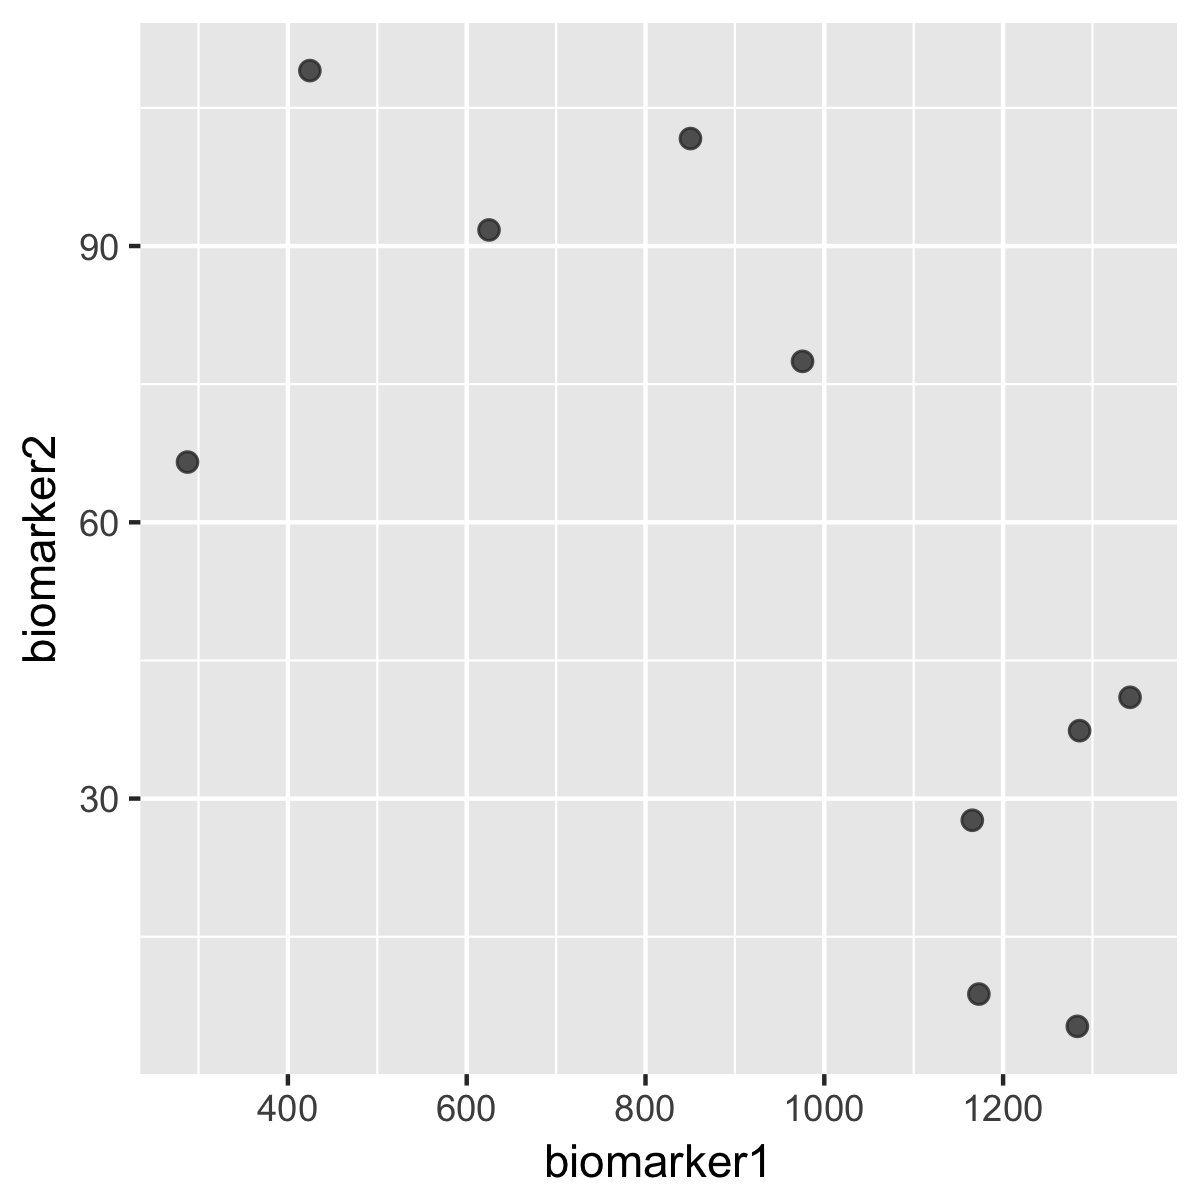
\includegraphics[width=0.47\textwidth]{img/biomarker-data-plain.png}
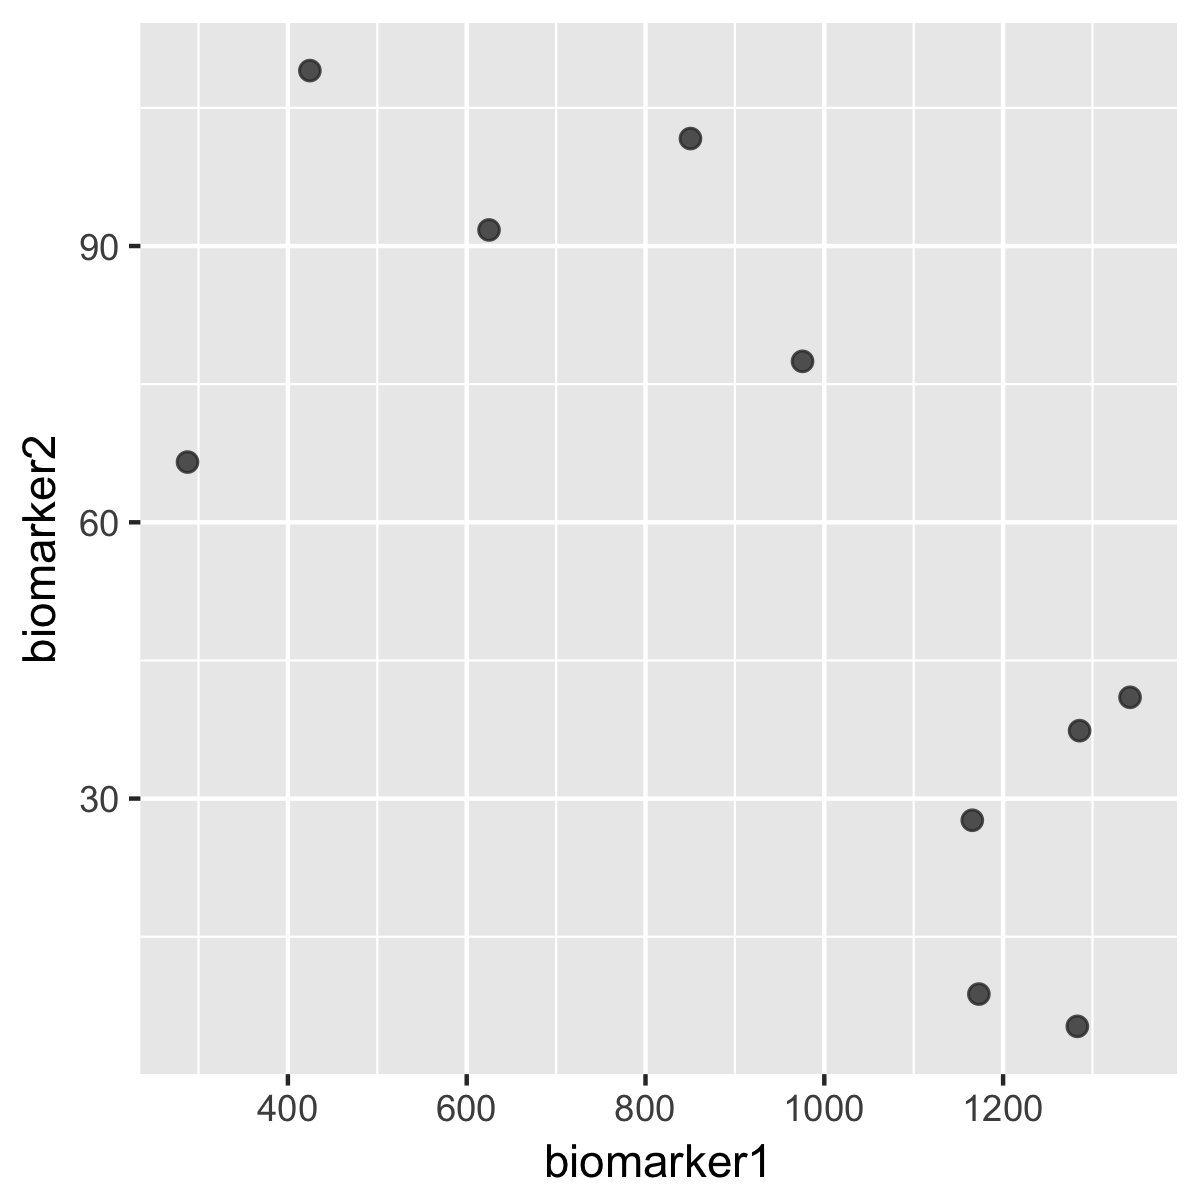
\includegraphics[width=0.47\textwidth]{img/biomarker-data-plain.png}
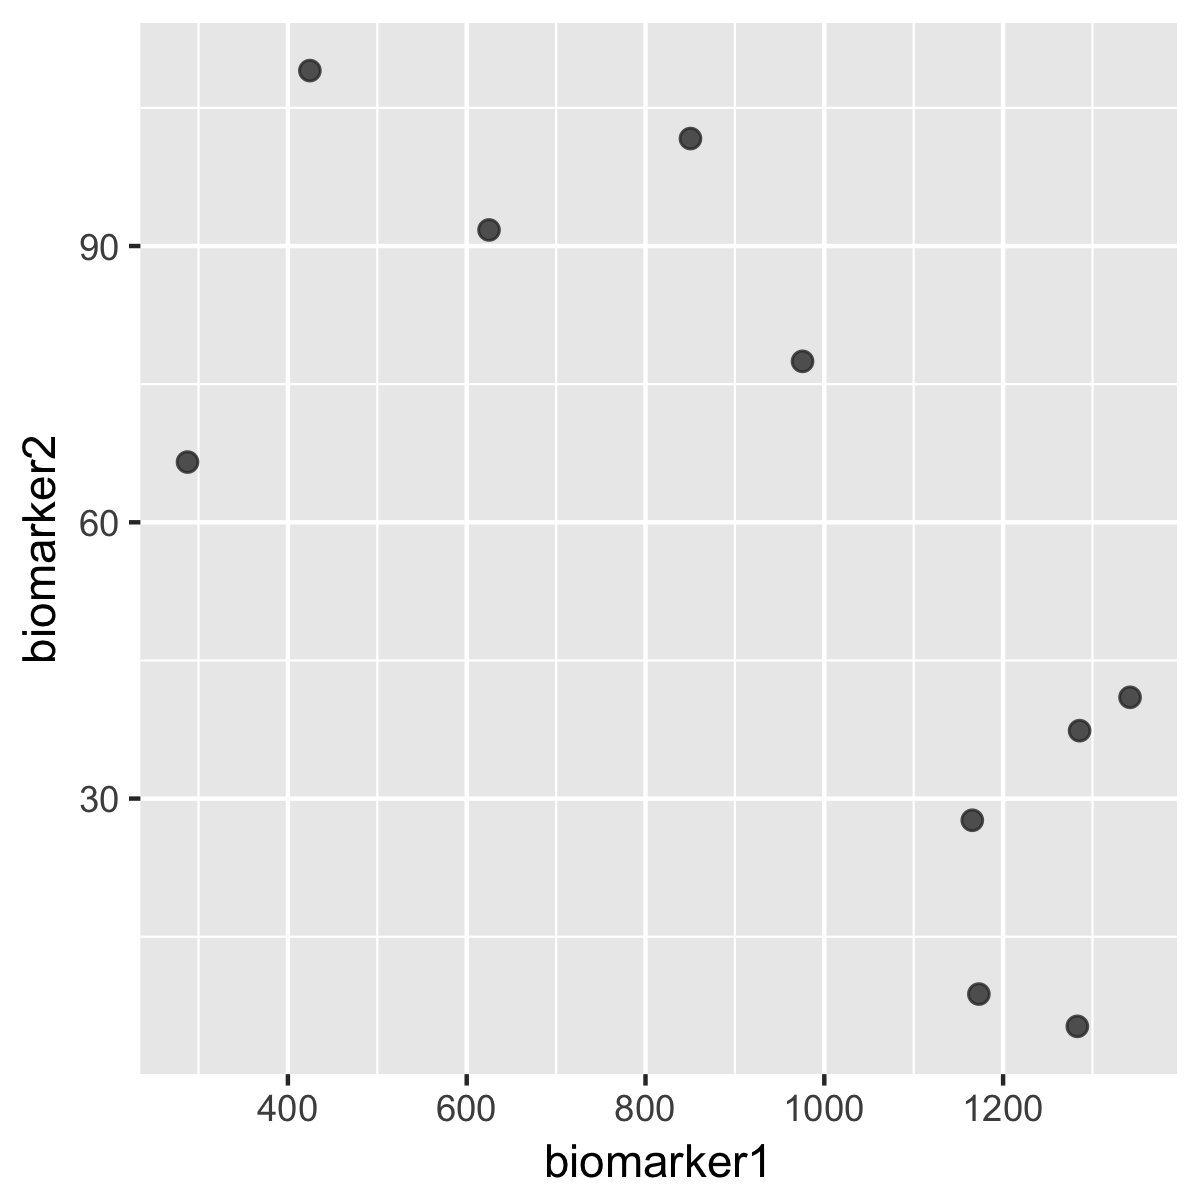
\includegraphics[width=0.47\textwidth]{img/biomarker-data-plain.png}
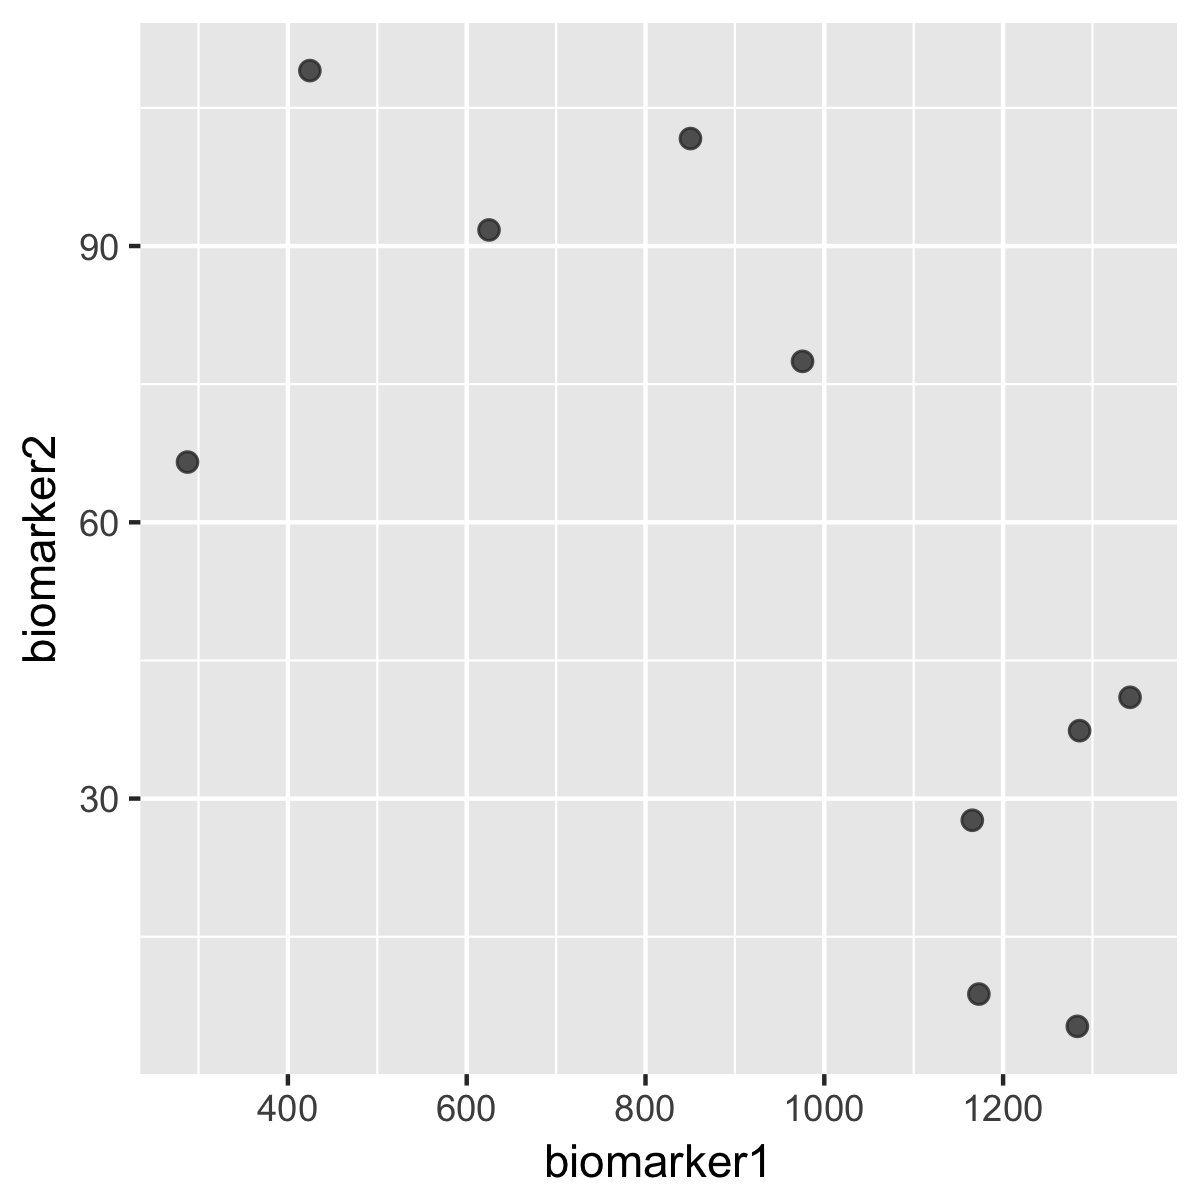
\includegraphics[width=0.47\textwidth]{img/biomarker-data-plain.png}
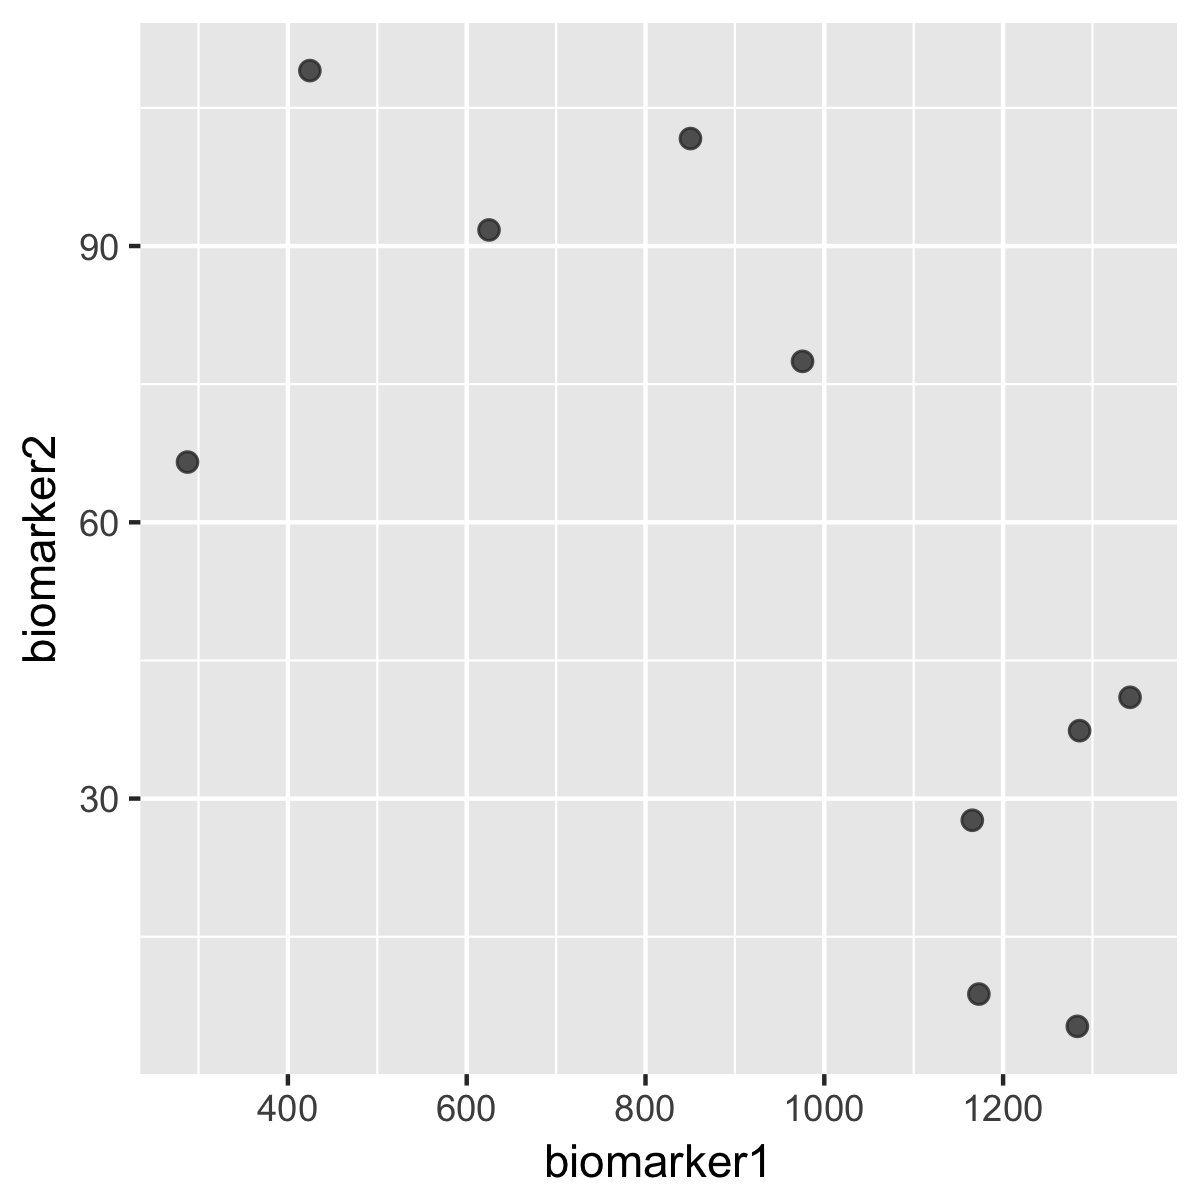
\includegraphics[width=0.47\textwidth]{img/biomarker-data-plain.png}
\end{center}
\end{question}

\begin{question}{}
What are some disadvantages of K-means?
\end{question}

\begin{question}{}
One application of K-means clustering is image compression, as shown in the figure below (which is from Christopher Bishop's classic book \emph{Pattern Recognition and Machine Learning}). 
\begin{center}
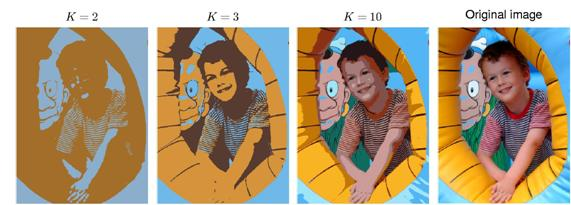
\includegraphics[width=0.8\textwidth]{img/cmm-bishop-kmeans.jpg}
\end{center}
Draw a picture of the data matrix for the image compression clustering problem. How will the clustering work here? Are we clustering rows or columns? What are the dimensions of the dataset, $n$ and $p$?
\end{question}

%%%%%%%%%%%%%%%%%%%%%%%%%%%%%%%%%%%%%%%%%%%%%%%%%%%%%%%%%%%%%%%%%%%

\section{Mixture Models \label{sect:mixturemodels}}

Mixture models represent data using mixtures of simple probability distributions. They are a step up in methodological rigor from $K$-means and are much more flexible, although the basic idea is the same. 

\noindent Here are the key similarities:

\begin{enumerate}
\item The number of clusters, $K$, is still an input parameter.
\item Mixture models can still converge to local minima depending on the initialization.
\end{enumerate}

\noindent Here are the key differences:

\begin{enumerate}
\item Mixture models use a \textbf{soft clustering} instead of a hard clustering. Each datapoint is assigned a probability distribution over potential clusters.
\item Instead of a distance metric like Euclidean distance, points are distributed over clusters by considering probability densities of the various clusters and how likely it is that the point came from each probability density.
\item No need to assume axes are on an equal scale; the individual probability distributions can account for this.
\end{enumerate}

We'll examine mixtures of Gaussians today because they're easy to visualize, but in reality the mixture components can be any type of well-behaved probability distribution.

%%%%%%%%%%%%%%%%%%%%%%%%%%%%%%%%%%%%%%%%%%%%%%%%%%%%%%%%%%%%%%%%%%%%%%%%%%%%%%%%

\section{Multivariate Gaussian Distribution}

We already saw the univariate Gaussian in Chapter~\ref{chapter:probabilitydistributions}. The \textbf{multivariate Gaussian} is an extension of the Gaussian to multiple dimensions.

\subsection{Probability Density and Parameters}

The $m$-dimensional \textbf{multivariate Gaussian} probability distribution is given by:
\begin{align*} p(x | \mu, \boldsymbol\Sigma)
&= \frac{1}{\sqrt{(2\pi)^m|\boldsymbol\Sigma|}}
\exp\left(-\frac{1}{2}({x}-{\mu})^T{\boldsymbol\Sigma}^{-1}({x}-{\mu})
\right) \end{align*}
where $x \in \mathbb{R}^m$ (a vector of length $m$) and the mean, $\mu$, is also a vector of length $m$. The variance of a univariate Gaussian, $\sigma$, is replaced by a covariance matrix of dimension $m \times m$:
$$ \boldsymbol\Sigma = \begin{bmatrix} \sigma_1^2 & \rho_{12}\sigma_1 \sigma_2 & \dots & \rho_{1m}\sigma_1 \sigma_m \\
\vdots & \vdots & \ddots & \vdots \\
\rho_{m1}\sigma_m \sigma_1 & \rho_{m2}\sigma_m \sigma_2 & \dots & \sigma_m^2 \end{bmatrix} $$
where $\rho_{ij}$ is the Pearson correlation of $X_i$ and $X_j$. Or alternatively, the $ij$th element of the covariance matrix is $\text{cov}(X_i, X_j) = E\left[ (X_i - \mu_i)(X_j - \mu_j) \right]$.

In two dimensions, the cross-sections of the multivariate Gaussian distribution are ellipses. The axes of the ellipses are given by the eigenvectors of the covariance matrix, $\boldsymbol\Sigma$. The first and second eigenvalues of the covariance matrix give the variance of the data along the major and minor axes of the ellipses, respectively. Some examples of bivariate normal distributions are shown below. This figure and the code that generated it can be found here:
\texttt{\small http://www.stat.cmu.edu/$\sim$kass/KEB/RHTML/R/bivariateNormalPerspectives.r.html}

\begin{center}
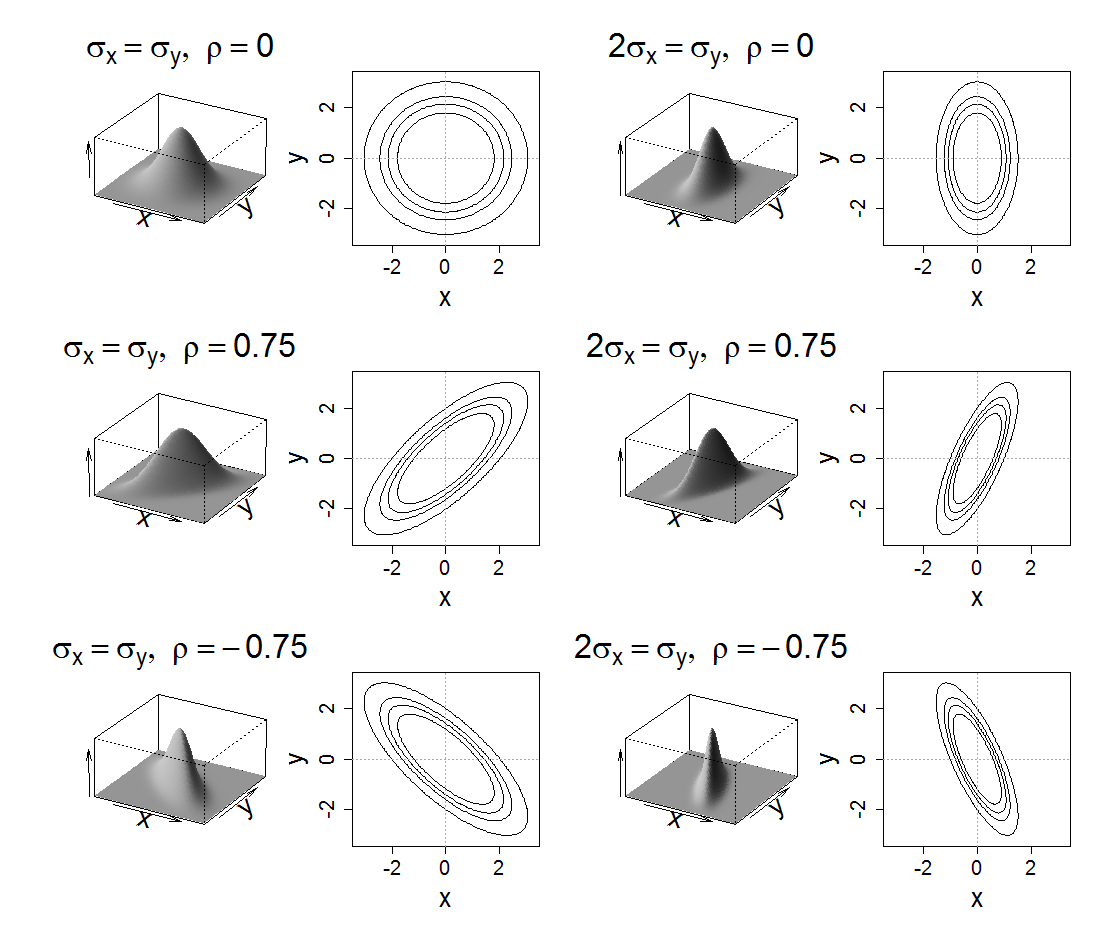
\includegraphics[width=0.9\textwidth]{img/bivariateNormalRev.png}
\end{center}

\subsection{Maximum Likelihood Estimates}

To fit data to a multivariate Gaussian distribution, we once again use our old friend, maximum likelihood estimation (Chapter~\ref{chapter:mlebasics}. Here are the maximum likelihood estimates for $\mu$ and $\boldsymbol{\Sigma}$ for the multivariate Gaussian:
\begin{align*} {\hat{\mu} = \frac{1}{n} \sum_{i=1}^n x^{(i)}} \qquad\qquad \hat{\boldsymbol\Sigma} = \frac{1}{n} \sum_{i=1}^n (x^{(i)}-\hat{\mu})(x^{(i)}-\hat{\mu})^T \end{align*}

%%%%%%%%%%%%%%%%%%%%%%%%%%%%%%%%%%%%%%%%%%%%%%%%%%%%%%%%%%%%%%%%%%%%%%%%%%%%%%%%

\section{Gaussian Mixture Models}

A Gaussian mixture model fits a set of unlabeled data to a set of $K$ multivariate Gaussians. There are three sets of parameters that the algorithm needs to identify:
\begin{enumerate}
\item $\mu_1, \dots, \mu_K$ (the means of the Gaussians)
\item $\boldsymbol\Sigma_1, \dots, \boldsymbol\Sigma_K$ (the covariance matrices of the Gaussians)
\item $\phi_1, \dots, \phi_K$ (the mixing proportions, which must sum to one)
\end{enumerate}

\vspace{1mm}

\begin{question}{question:flowcode}
Mixture models are examples of \textbf{generative models}, which tell a story about how the observed data were generated. Below is the actual code that generated the data for the flow cytometry example.
\begin{center}
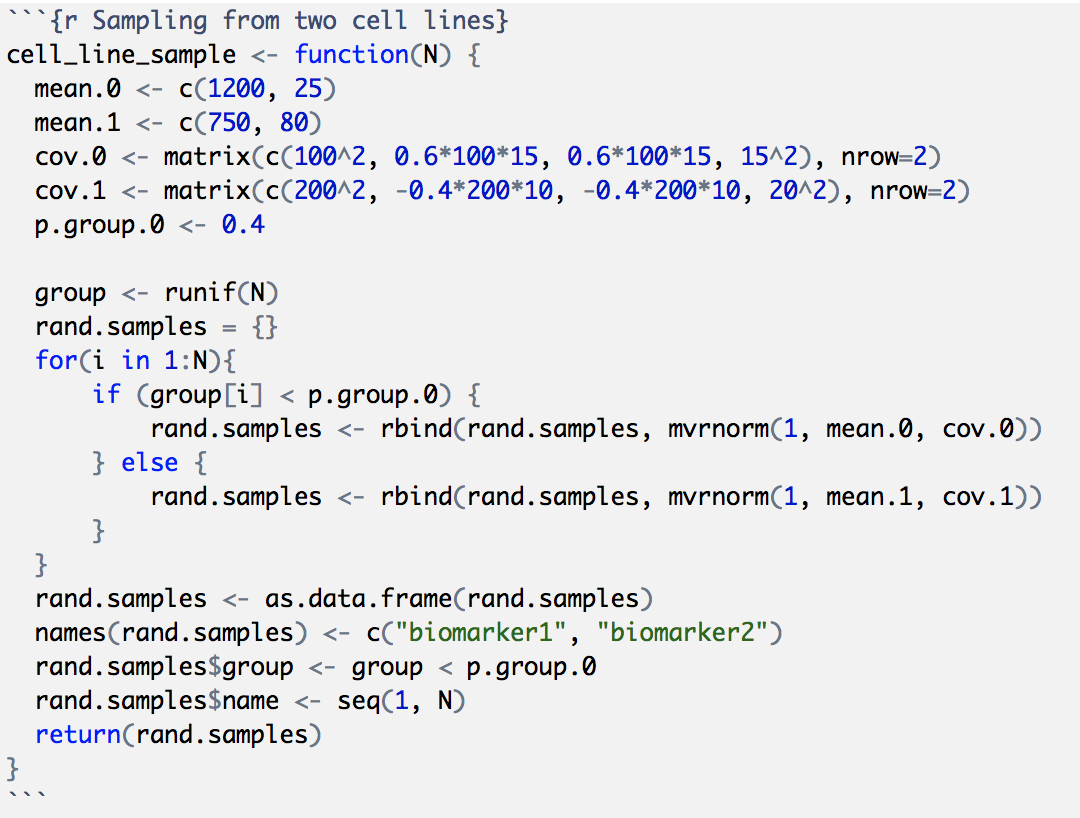
\includegraphics[width=0.85\textwidth]{img/biomarker-code.png}
\end{center}
It turns out that this code matches the ``story'' of the Gaussian mixture model perfectly. (With real data, of course, this would not be the case.) What is that story?
\end{question}

\noindent Here is the algorithm for fitting a Gaussian mixture model:
\begin{enumerate}
\item Initialize the means $\mu_k$, covariances $\boldsymbol\Sigma_k$, and mixing coefficients $\phi_k$ for all of the Gaussians $k=1,\dots,K$.

\item \textbf{E step.} Give each point a ``voting weight'' in each Gaussian equal to the probability (based on current parameter values) that it came from that Gaussian:
\begin{align*} w_j^{(i)} &:= p(z^{(i)} = j | x^{(i)}, \phi, \mu, \boldsymbol\Sigma) \\
&= \frac{\phi_j \cdot \mathcal{N}(x^{(i)}|\mu_j, \boldsymbol\Sigma_j)}{\sum_{k=1}^K \phi_k \cdot \mathcal{N}(x^{(i)}|\mu_k, \boldsymbol\Sigma_k)} \end{align*}
Note that you will have $K$ different voting weights for each point, and there are $n$ points, so you need to do $nK$ total calculations here.

\item \textbf{M step.} Re-estimate the parameters for the different Gaussians by letting each point vote in each Gaussian according to its voting weight.
\begin{align*}
\phi_j &:= \frac{1}{n} \sum_{i=1}^n w_j^{(i)} \\
\mu_j &:= \cfrac{\sum_{i=1}^n w_j^{(i)} x^{(i)}}{\sum_{i=1}^n w_j^{(i)}} \\
\boldsymbol\Sigma_j &:= \cfrac{\sum_{i=1}^n w_j^{(i)} (x^{(i)} - \mu_j)(x^{(i)} - \mu_j)^T}{\sum_{i=1}^n w_j^{(i)}}
\end{align*}
\item Check for convergence of either the parameters or the log-likelihood. If the convergence criterion is not satisfied, return to step 2.
\end{enumerate}

Note that you are \emph{not} guaranteed to get the right answer; the final Gaussians can change depending on how you initialize the model. 

%%%%%%%%%%%%%%%%%%%%%%%%%%%%%%%%%%%%%%%%%%%%%%%%%%%%%%%%%%%%%%%%%%%%%%%%%%%%%%%%

\section{A Gaussian Mixture Model for Flow Cytometry Data}

We will now follow the steps from the algorithm above to fit a Gaussian mixture model to the dataset from our flow cytometry example.

\begin{enumerate}
\item Initialize the means $\mu_A$ and $\mu_B$, the covariances $\boldsymbol\Sigma_A$ and $\boldsymbol\Sigma_B$, and the mixing coefficients $\phi_A$ and $\phi_B$. 

\begin{minipage}[t]{0.45\textwidth}
\begin{center}
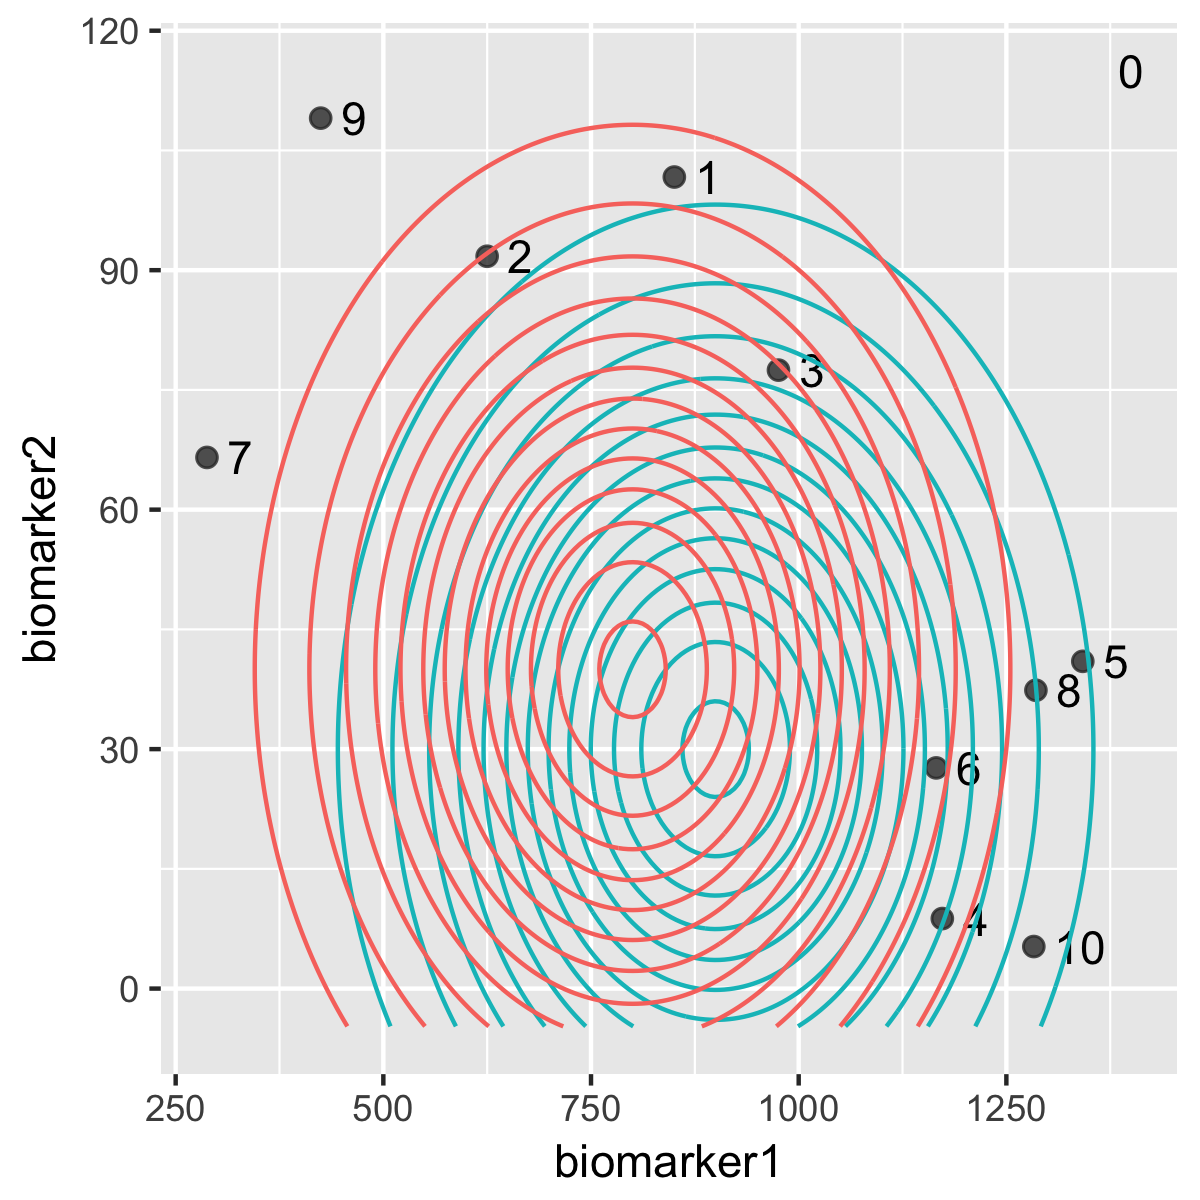
\includegraphics[scale=0.15]{img/biomarker-data-labels-0.png}
\end{center}
\end{minipage}
\qquad
\begin{minipage}[t]{0.45\textwidth}
\small
\begin{align*} 
\phi_A &= 0.5 \\
\phi_B &= 0.5 \\
\mu_A &= \begin{bmatrix} 900 \\ 30 \end{bmatrix} \\
\mu_B &= \begin{bmatrix} 800 \\ 40 \end{bmatrix} \\
\boldsymbol\Sigma_A &= \begin{bmatrix} 200^2 & 0 \\ 0 & 30^2 \end{bmatrix} \\
\boldsymbol\Sigma_B &= \begin{bmatrix} 200^2 & 0 \\ 0 & 30^2 \end{bmatrix}
\end{align*}
\end{minipage}

\vspace{10mm}

\item Do E step for round 1.

\begin{center}
\small
\begin{tabular}{crrcccc}
\toprule
$i$ & $x_1^{(i)}$ & $x_2^{(i)}$ & $\mathcal{N}(x^{(i)}| \mu_A, \boldsymbol\Sigma_A)$ & $\mathcal{N}(x^{(i)}|\mu_B, \boldsymbol\Sigma_B)$ & $w_A^{(i)}$ & $w_B^{(i)}$ \\
\midrule
1 & 634.83 & 110.55 & 3e-07 & 1.2e-06 & 0.201 & 0.799 \\ 
  2 & 650.06 & 74.22 & 4.1e-06 & 1e-05 & 0.282 & 0.718 \\ 
  3 & 788.24 & 81.52 & 5.2e-06 & 1e-05 & 0.338 & 0.662 \\ 
  4 & 771.47 & 84.98 & 4e-06 & 8.5e-06 & 0.320 & 0.680 \\ 
  5 & 515.81 & 91.08 & 5.3e-07 & 2.3e-06 & 0.189 & 0.811 \\ 
  6 & 1101.23 & 31.05 & 1.6e-05 & 8.2e-06 & 0.662 & 0.338 \\ 
  7 & 649.32 & 77.05 & 3.5e-06 & 9.3e-06 & 0.275 & 0.725 \\ 
  8 & 652.89 & 97.16 & 1e-06 & 3.3e-06 & 0.234 & 0.766 \\ 
  9 & 1183.02 & 11.73 & 8.1e-06 & 2.7e-06 & 0.749 & 0.251 \\ 
  10 & 1238.45 & 33.46 & 6.3e-06 & 2.3e-06 & 0.729 & 0.271 \\ 
\midrule
sum & & & & & 3.979 & 6.021 \\
\bottomrule
\end{tabular}
\end{center}

\vspace{5mm}

\item Do M step for round 1.

\begin{minipage}[t]{0.45\textwidth}
\begin{center}
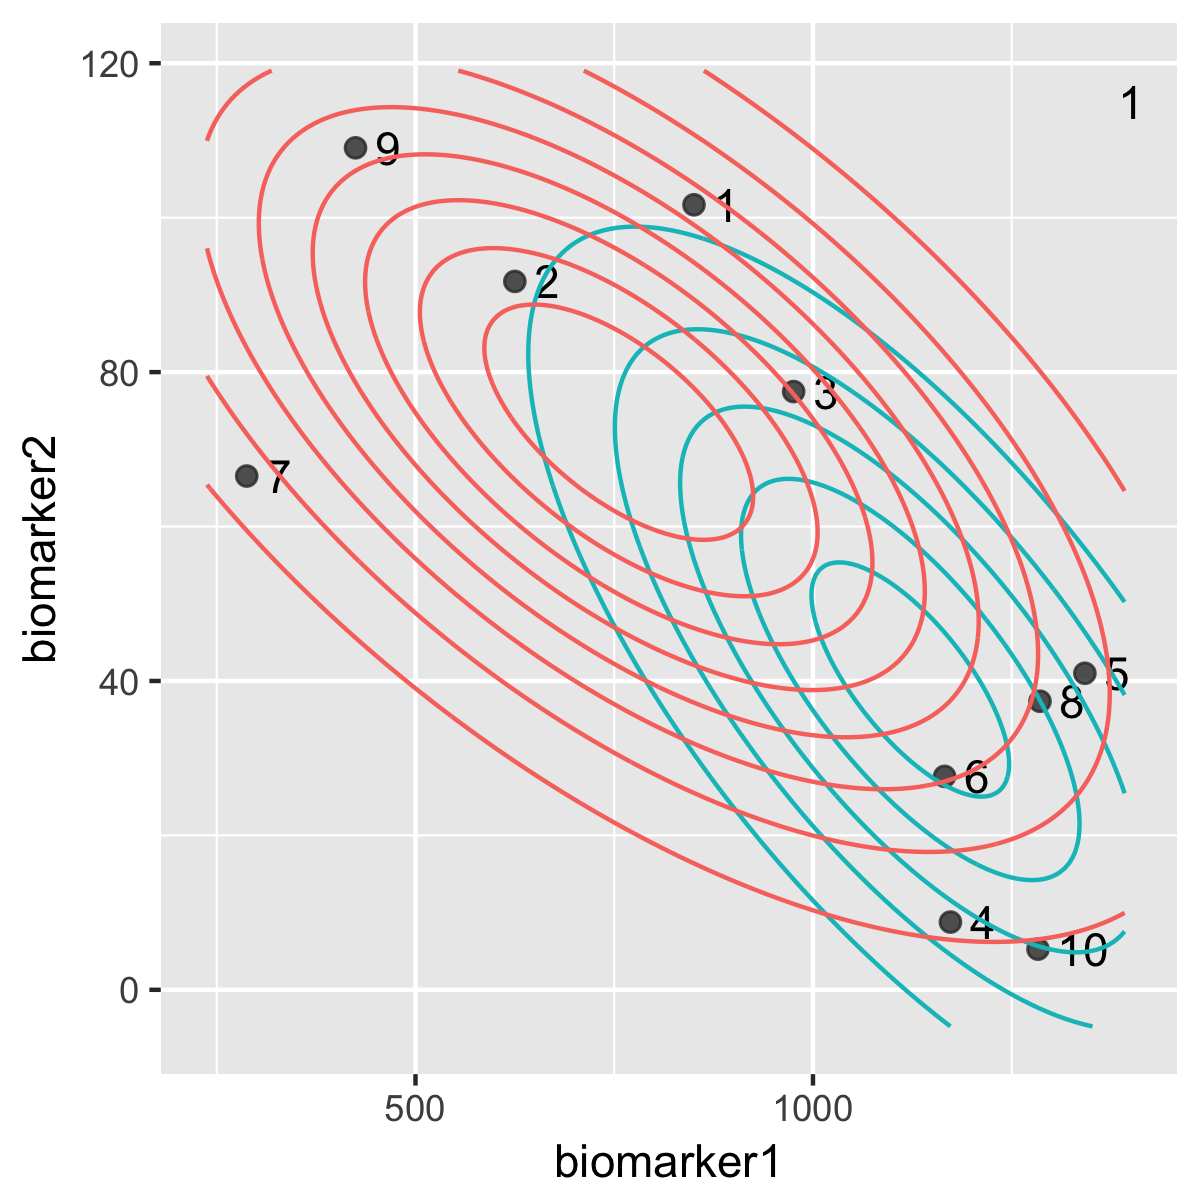
\includegraphics[scale=0.15]{img/biomarker-data-labels-1.png}
\end{center}
\end{minipage}
\qquad
\begin{minipage}[t]{0.45\textwidth}
\small
\begin{align*} 
\phi_A &= 0.398 \\
\phi_B &= 0.602 \\
\mu_A &= \begin{bmatrix} 947.6 \\ 53.5 \end{bmatrix} \\
\mu_B &= \begin{bmatrix} 733.2 \\ 79.7 \end{bmatrix} \\
\boldsymbol\Sigma_A &= \begin{bmatrix} 256.6^2 & -0.925 \cdot 256.6 \cdot 32.3 \\ -0.925 \cdot 256.6 \cdot 32.3 & 32.3^2 \end{bmatrix} \\
\boldsymbol\Sigma_B &= \begin{bmatrix} 195.4^2 & -0.855 \cdot 195.4 \cdot 24.7 \\ -0.855 \cdot 195.4 \cdot 24.7 & 24.7^2\end{bmatrix} 
\end{align*}
\end{minipage}

\vspace{10mm}

\item Do E step for round 2.

\begin{center}
\small
\begin{tabular}{crrcccc}
\toprule
$i$ & $x_1^{(i)}$ & $x_2^{(i)}$ & $\mathcal{N}(x^{(i)}| \mu_A, \boldsymbol\Sigma_A)$ & $\mathcal{N}(x^{(i)}|\mu_B, \boldsymbol\Sigma_B)$ & $w_A^{(i)}$ & $w_B^{(i)}$ \\
\midrule
1 & 634.83 & 110.55 & 5.9e-06 & 1.6e-05 & 0.193 & 0.807 \\ 
  2 & 650.06 & 74.22 & 1.4e-05 & 3.1e-05 & 0.226 & 0.774 \\ 
  3 & 788.24 & 81.52 & 3.1e-05 & 5.1e-05 & 0.287 & 0.713 \\ 
  4 & 771.47 & 84.98 & 2.7e-05 & 4.8e-05 & 0.271 & 0.729 \\ 
  5 & 515.81 & 91.08 & 7.2e-06 & 2.2e-05 & 0.178 & 0.822 \\ 
  6 & 1101.23 & 31.05 & 3.9e-05 & 8.5e-06 & 0.754 & 0.246 \\ 
  7 & 649.32 & 77.05 & 1.7e-05 & 3.8e-05 & 0.227 & 0.773 \\ 
  8 & 652.89 & 97.16 & 2e-05 & 4.6e-05 & 0.219 & 0.781 \\ 
  9 & 1183.02 & 11.73 & 1.7e-05 & 1.5e-06 & 0.884 & 0.116 \\ 
  10 & 1238.45 & 33.46 & 1.4e-05 & 1.8e-06 & 0.837 & 0.163 \\ 
\midrule
sum & & & & & 4.078 & 5.922 \\
\bottomrule
\end{tabular}
\end{center}

\newpage

\item Do M step for round 2. Calculate the new log-likelihood.

\begin{minipage}[t]{0.45\textwidth}
\begin{center}
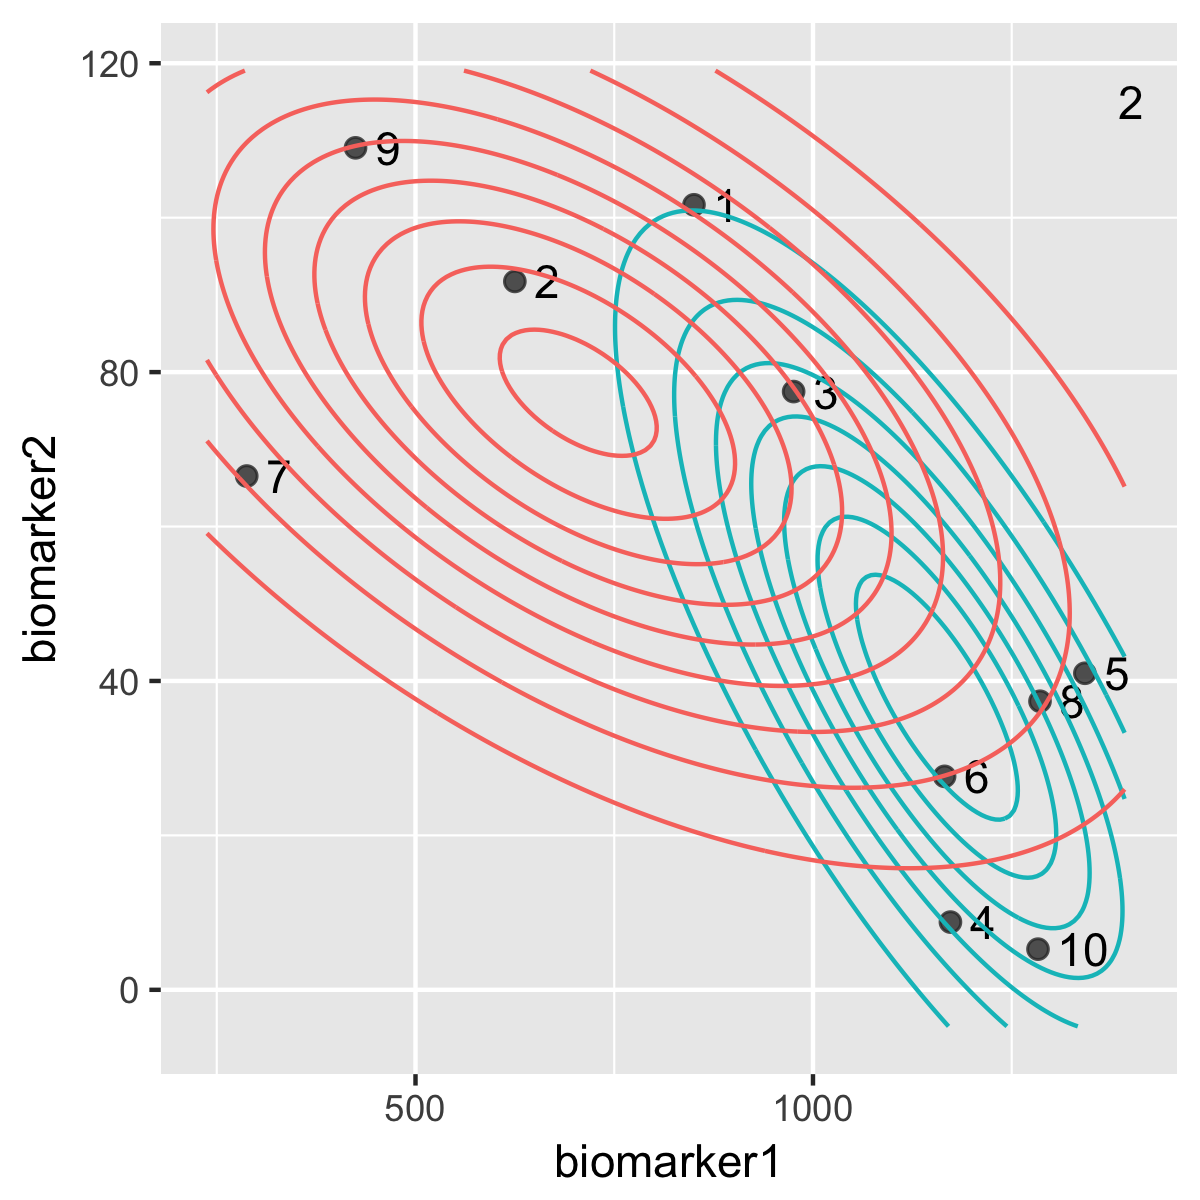
\includegraphics[scale=0.15]{img/biomarker-data-labels-2.png}
\end{center}
\end{minipage}
\qquad
\begin{minipage}[t]{0.45\textwidth}
\small
\begin{align*} 
\phi_A &= 0.408 \\
\phi_B &= 0.592 \\
\mu_A &= \begin{bmatrix} 981.2 \\ 49.4 \end{bmatrix} \\
\mu_B &= \begin{bmatrix} 706.5 \\ 83 \end{bmatrix} \\
\boldsymbol\Sigma_A &= \begin{bmatrix} 252.6^2 & -0.924 \cdot 252.6 \cdot 32.1 \\ -0.924 \cdot 252.6 \cdot 32.1 & 32.1^2 \end{bmatrix} \\
\boldsymbol\Sigma_B &= \begin{bmatrix} 164.3^2 & -0.793 \cdot 164.3 \cdot 20.8 \\ -0.793 \cdot 164.3 \cdot 20.8 & 20.8^2 \end{bmatrix} 
\end{align*}
\end{minipage}

\vspace{10mm}

\item Do E step for round 3.

\begin{center}
\small
\begin{tabular}{crrcccc}
\toprule
$i$ & $x_1^{(i)}$ & $x_2^{(i)}$ & $\mathcal{N}(x^{(i)}| \mu_A, \boldsymbol\Sigma_A)$ & $\mathcal{N}(x^{(i)}|\mu_B, \boldsymbol\Sigma_B)$ & $w_A^{(i)}$ & $w_B^{(i)}$ \\
\midrule
1 & 634.83 & 110.55 & 5e-06 & 1.9e-05 & 0.153 & 0.847 \\ 
  2 & 650.06 & 74.22 & 1.1e-05 & 3.8e-05 & 0.171 & 0.829 \\ 
  3 & 788.24 & 81.52 & 2.8e-05 & 5.9e-05 & 0.250 & 0.750 \\ 
  4 & 771.47 & 84.98 & 2.4e-05 & 5.6e-05 & 0.230 & 0.770 \\ 
  5 & 515.81 & 91.08 & 5.4e-06 & 2.7e-05 & 0.122 & 0.878 \\ 
  6 & 1101.23 & 31.05 & 4.3e-05 & 2.7e-06 & 0.917 & 0.083 \\ 
  7 & 649.32 & 77.05 & 1.4e-05 & 4.7e-05 & 0.171 & 0.829 \\ 
  8 & 652.89 & 97.16 & 1.7e-05 & 5.7e-05 & 0.167 & 0.833 \\ 
  9 & 1183.02 & 11.73 & 2e-05 & 2.1e-07 & 0.985 & 0.015 \\ 
  10 & 1238.45 & 33.46 & 1.6e-05 & 3.8e-07 & 0.965 & 0.035 \\
\midrule
sum & & & & & 4.132 & 5.868 \\
\bottomrule
\end{tabular}
\end{center}

\newpage

\item Do M step for round 3.

\begin{minipage}[t]{0.45\textwidth}
\begin{center}
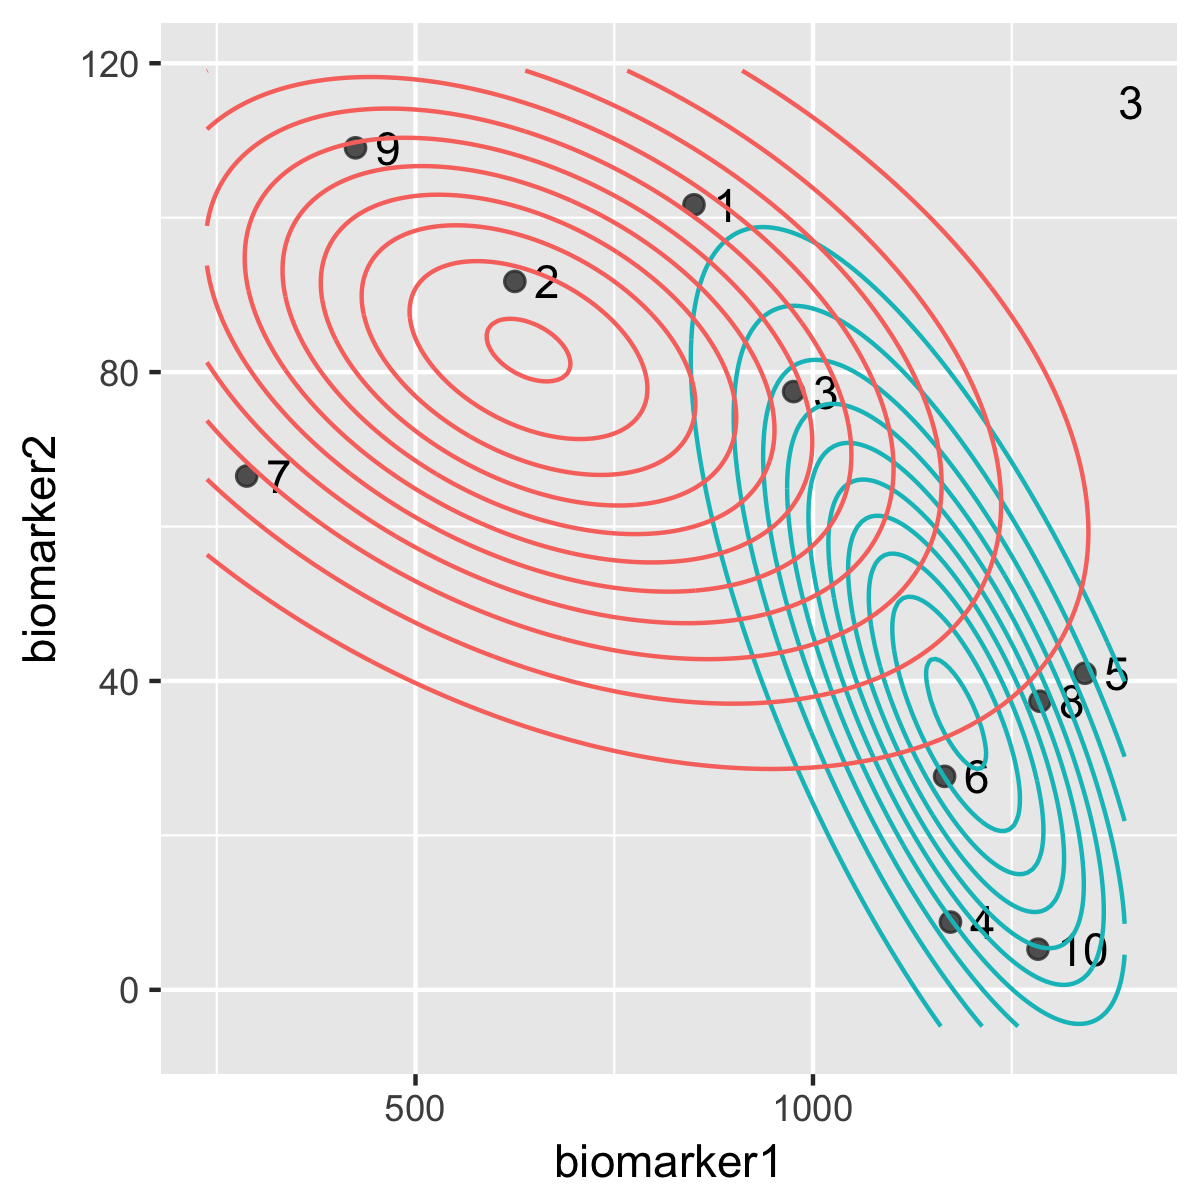
\includegraphics[scale=0.15]{img/biomarker-data-labels-3.png}
\end{center}
\end{minipage}
\qquad
\begin{minipage}[t]{0.45\textwidth}
\small
\begin{align*} 
\phi_A &= 0.413 \\
\phi_B &= 0.587 \\
\mu_A &= \begin{bmatrix} 1025.3 \\ 44.2 \end{bmatrix} \\
\mu_B &= \begin{bmatrix} 672.9 \\ 87 \end{bmatrix} \\
\boldsymbol\Sigma_A &= \begin{bmatrix} 235.5^2 & -0.916 \cdot 235.5 \cdot 30.3 \\ -0.916 \cdot 235.5 \cdot 30.3 & 30.3^2 \end{bmatrix} \\
\boldsymbol\Sigma_B &= \begin{bmatrix} 110.6^2 & -0.558 \cdot 110.6 \cdot 14.6 \\ -0.558 \cdot 110.6 \cdot 14.6 & 14.6^2 \end{bmatrix} 
\end{align*}
\end{minipage}

\vspace{10mm}

\item Do EM rounds 4 through 9.

\begin{center}
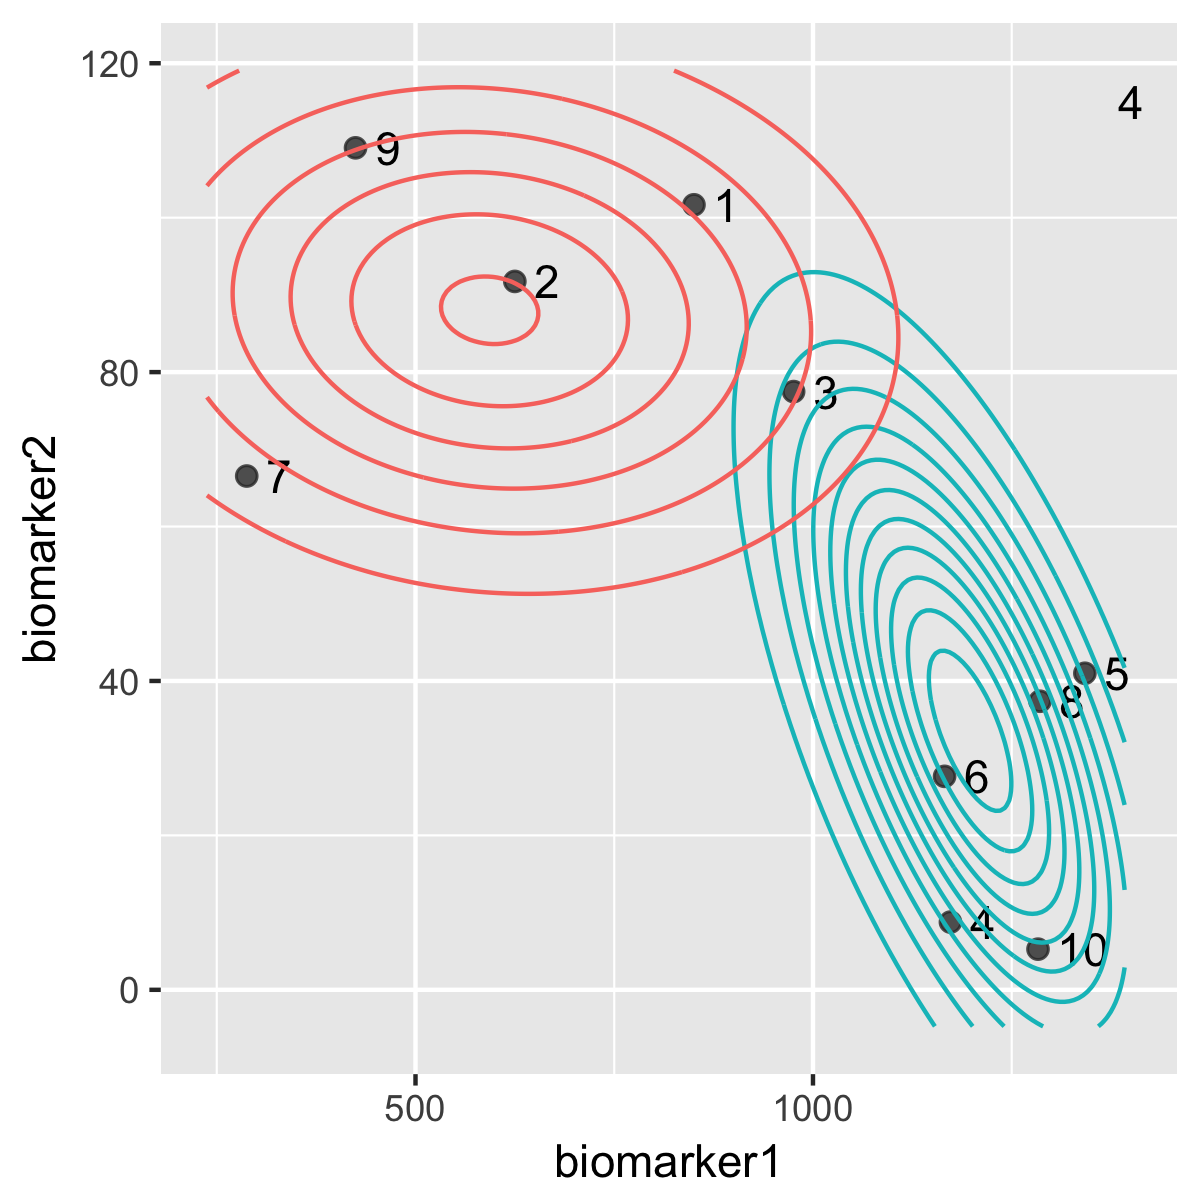
\includegraphics[width=0.45\textwidth]{img/biomarker-data-labels-4.png}
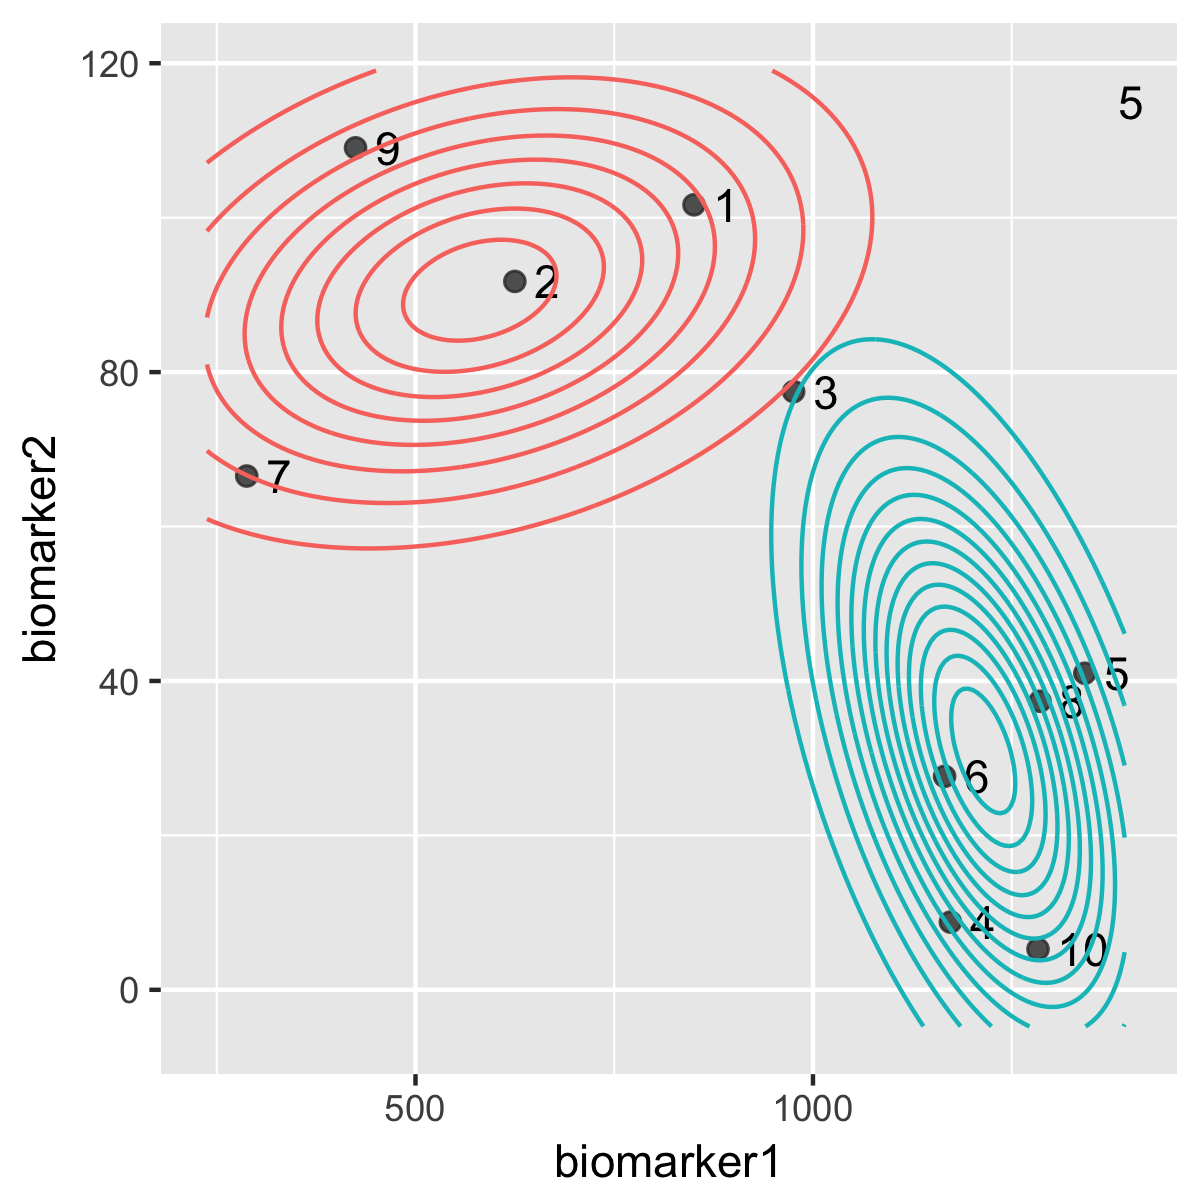
\includegraphics[width=0.45\textwidth]{img/biomarker-data-labels-5.png}
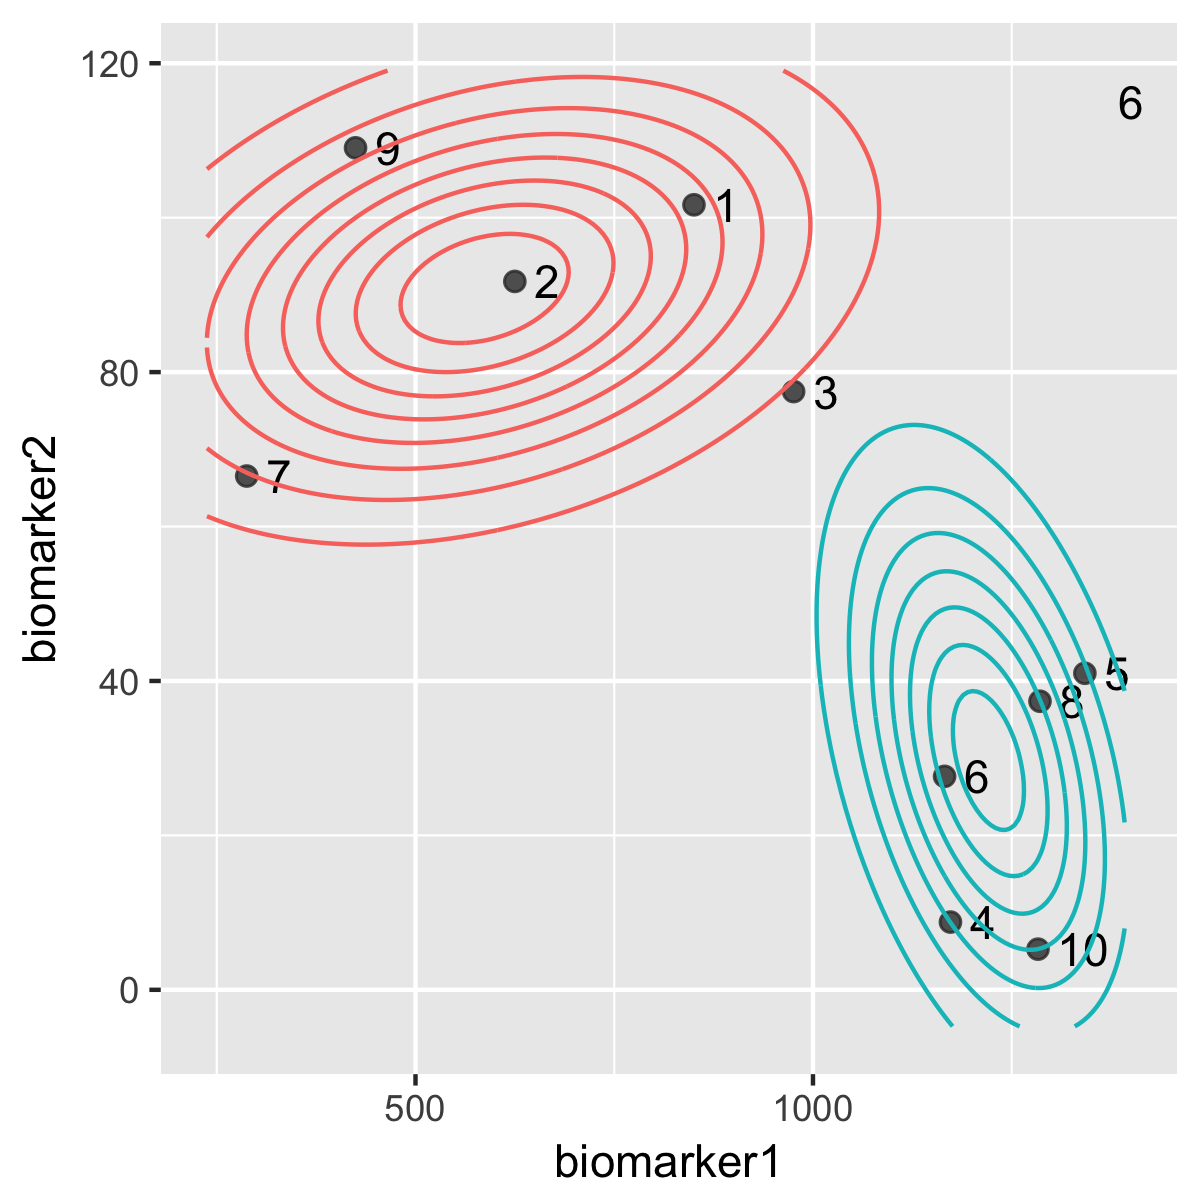
\includegraphics[width=0.45\textwidth]{img/biomarker-data-labels-6.png}
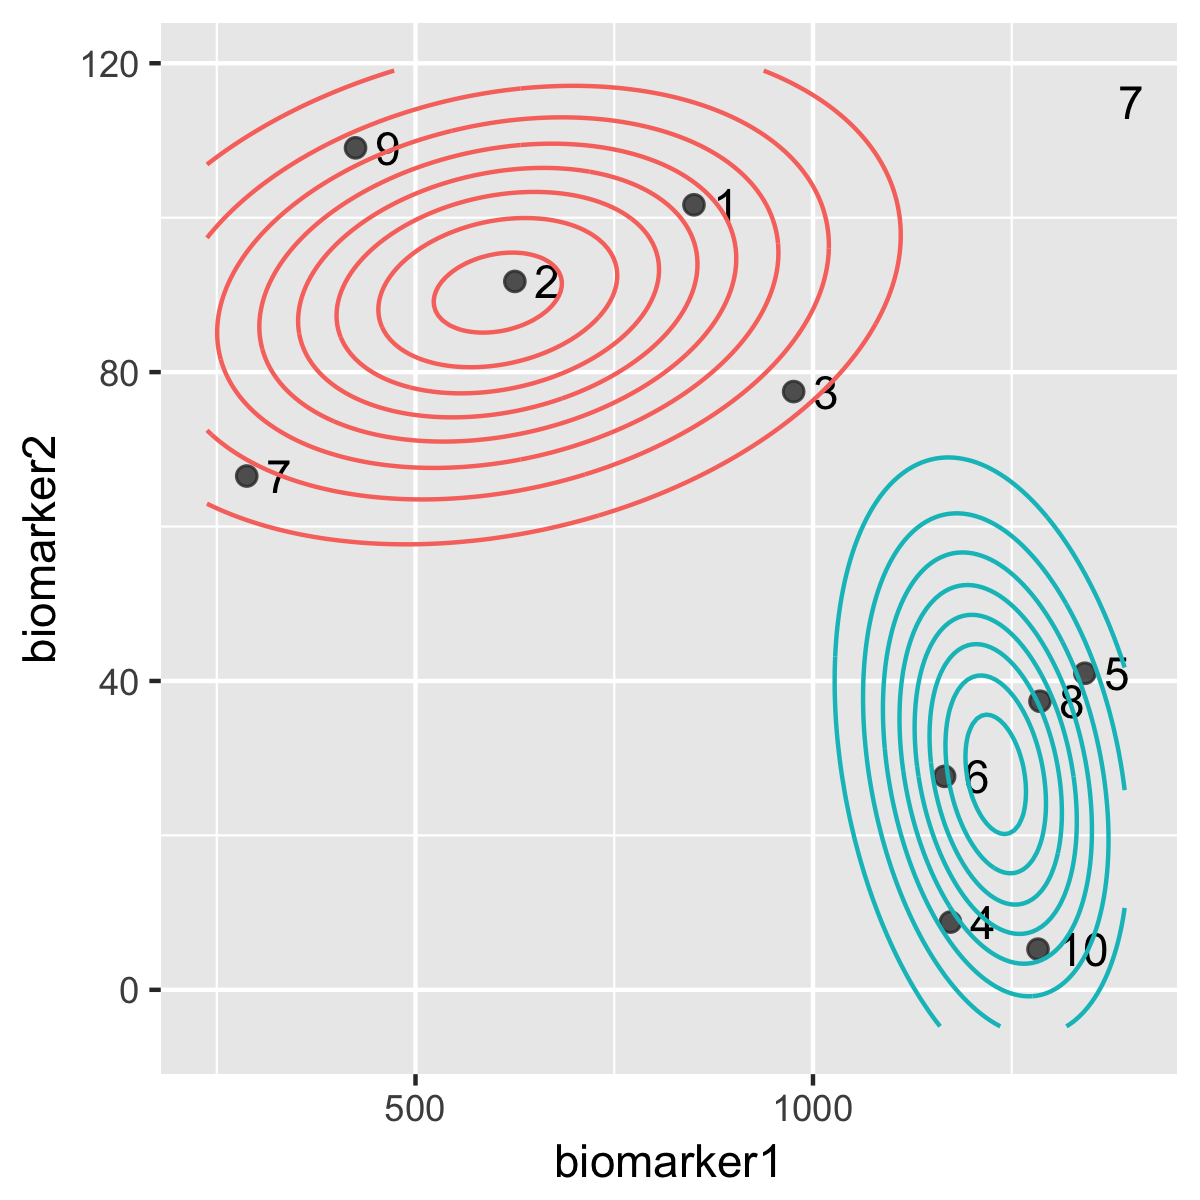
\includegraphics[width=0.45\textwidth]{img/biomarker-data-labels-7.png}
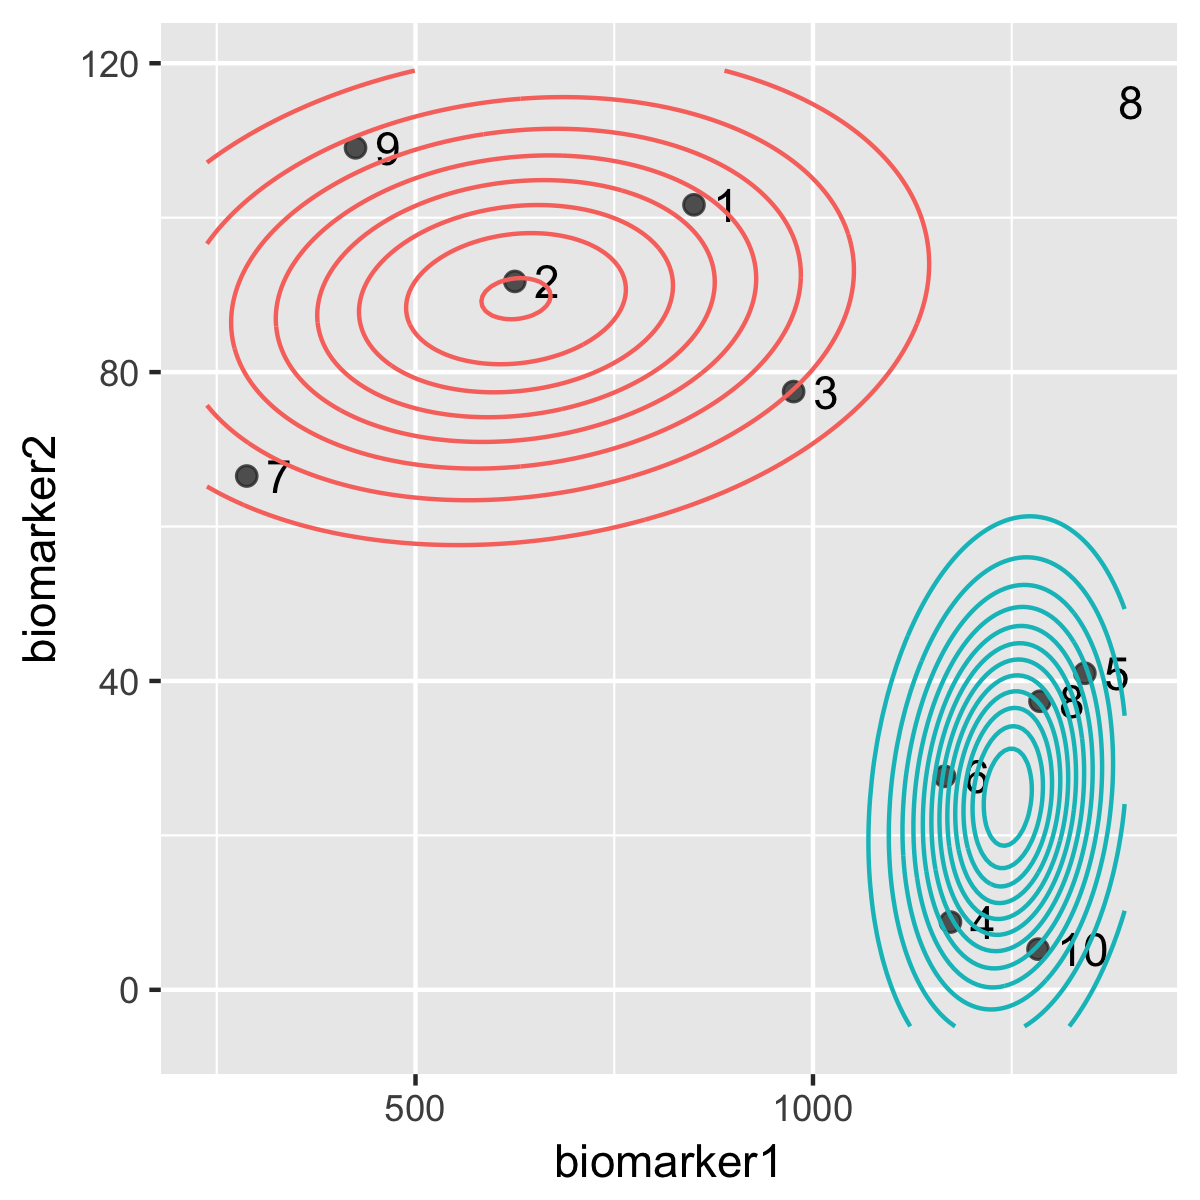
\includegraphics[width=0.45\textwidth]{img/biomarker-data-labels-8.png}
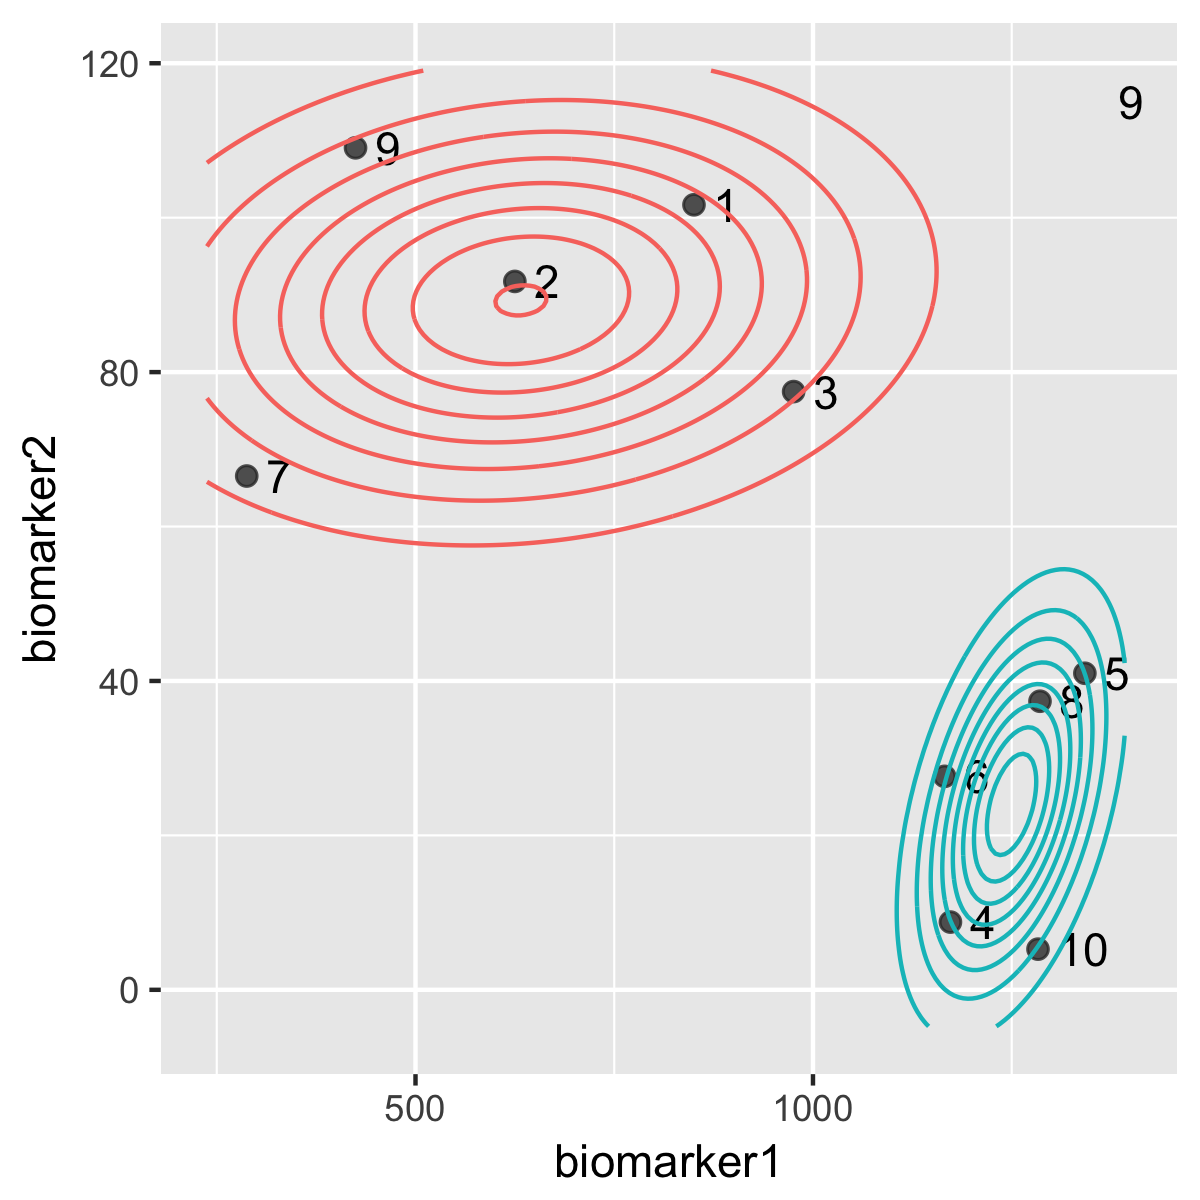
\includegraphics[width=0.45\textwidth]{img/biomarker-data-labels-9.png}
\end{center}

\end{enumerate}

\noindent Here is the table of calculations for the E-step after round 9:
\begin{center}
\small
\begin{tabular}{crrcccc}
\toprule
$i$ & $x_1^{(i)}$ & $x_2^{(i)}$ & $\mathcal{N}(x^{(i)}| \mu_A, \boldsymbol\Sigma_A)$ & $\mathcal{N}(x^{(i)}|\mu_B, \boldsymbol\Sigma_B)$ & $w_A^{(i)}$ & $w_B^{(i)}$ \\
\midrule
1 & 634.83 & 110.55 & 1.8e-40 & 2.6e-05 & 0.000 & 1.000 \\ 
  2 & 650.06 & 74.22 & 2.5e-28 & 7.1e-05 & 0.000 & 1.000 \\ 
  3 & 788.24 & 81.52 & 1.6e-21 & 5.8e-05 & 0.000 & 1.000 \\ 
  4 & 771.47 & 84.98 & 2.5e-23 & 7.7e-05 & 0.000 & 1.000 \\ 
  5 & 515.81 & 91.08 & 1.7e-43 & 3.4e-05 & 0.000 & 1.000 \\ 
  6 & 1101.23 & 31.05 & 0.00011 & 6e-13 & 1.000 & 0.000 \\ 
  7 & 649.32 & 77.05 & 5e-29 & 9.5e-05 & 0.000 & 1.000 \\ 
  8 & 652.89 & 97.16 & 2.2e-34 & 0.00012 & 0.000 & 1.000 \\ 
  9 & 1183.02 & 11.73 & 0.00011 & 6e-18 & 1.000 & 0.000 \\ 
  10 & 1238.45 & 33.46 & 0.00011 & 3.7e-16 & 1.000 & 0.000 \\   
\midrule
sum & & & & & 3.000 & 7.000 \\
\bottomrule
\end{tabular}
\end{center}

\noindent The values of the final parameters are:
\begin{align*} 
\phi_A &= 0.30 \\
\phi_B &= 0.70 \\
\mu_A &= \begin{bmatrix} 1174.2 \\ 25.4 \end{bmatrix} \\
\mu_B &= \begin{bmatrix} 666.1 \\ 88.1 \end{bmatrix} \\
\boldsymbol\Sigma_A &= \begin{bmatrix} 56.4^2 & -0.009 \cdot 56.4 \cdot 9.7 \\ -0.009 \cdot 56.4 \cdot 9.7 & 9.7^2  \end{bmatrix} \\
&= \begin{bmatrix} 3176.8 & -5.0 \\ -5.0 & 94.6 \end{bmatrix} \\
\boldsymbol\Sigma_B &= \begin{bmatrix} 84.8^2 & -0.287 \cdot 84.8 \cdot 11.7 \\ -0.287 \cdot 84.8 \cdot 11.7 & 11.7^2  \end{bmatrix} \\
&= \begin{bmatrix} 7185.8 & -284.8 \\ -284.8 & 137.5 \end{bmatrix}
\end{align*}

\begin{question}{}
Compare these parameters to the values from the code that generated the data (Question~\ref{question:flowcode}). What do you notice? 
\end{question}

\begin{question}{}
Think of 2-3 different unsupervised learning problems from biology or medicine where a mixture model makes sense, conceptually at least, for modeling the data. How would you set up the mixture model in each case?
\end{question}

%%%%%%%%%%%%%%%%%%%%%%%%%%%%%%%%%%%%%%%%%%%%%%%%%%%%%%%%%%%%%%%%%%%%%%%%%%%%%%%

\section{The Expectation-Maximization Algorithm}

Given a joint distribution $p(x, z|\theta)$ over observed variables $X$ and latent variables $Z$, governed by parameters $\theta$, the goal of the EM algorithm is to maximize the likelihood function $p(x|\theta)$ with respect to $\theta$. Mixture models are an example of the EM algorithm. Here is its general form:
\begin{enumerate}
\item Choose an initial setting for the parameters $\theta$.
\item \textbf{E step.} For each $i$, set
$$ Q_i (z^{(i)}) := p(z^{(i)}|x^{(i)}, \theta) $$
\item \textbf{M step.} Set
$$ \theta := \text{arg} \max_\theta \sum_{i=1}^n \sum_{z^{(i)}} Q_i (z^{(i)}) \log \frac{p(x^{(i)}, z^{(i)}|\theta)}{Q_i(z^{(i)})} $$
\item Check for convergence of either the log likelihood or the parameter values. If the convergence criterion is not satisfied, return to step 2.
\end{enumerate}

Why does this work? See Andrew Ng's lecture notes on the EM algorithm from CS229 at Stanford -- they contain the clearest explanation I've seen and use the same notation as us.

%%%%%%%%%%%%%%%%%%%%%%%%%%%%%%%%%%%%%%%%%%%%%%%%%%%%%%%%%%%%%%%%%%%%%%%%%%%%%%%

\section{Extensions}

There are many different clustering algorithms. You can find a good summary of all the different ones here: https://en.wikipedia.org/wiki/Cluster\_analysis. Some topics you might choose to investigate independently (or that we might look at together in the future) include:

\begin{itemize}
\item Hierarchical clustering (e.g. phylogenetic trees)
\item Methods for choosing $K$ (the number of clusters)
\item Bayesian methods that introduce priors on the parameters in mixture models
\item Biclustering
\end{itemize}

There are also many different types of mixture models that all use the EM algorithm for maximum likelihood optimization. You may want to check out the following (and many more):

\begin{itemize}
\item Hidden Markov Models (Baum-Welch algorithm)
\item Inside-outside algorithm for induction of probabilistic context-free grammars 
\item Leicht and Newman's 2007 PNAS paper on finding network clusters using mixture models
\item Alignment algorithms for genetic sequence data using HMMs
\end{itemize}

